\documentclass[
11pt,
tightenlines,
twoside,
onecolumn,
nofloats,
nobibnotes,
nofootinbib,
superscriptaddress,
noshowpacs,
centertags]
{revtex4-2}
\usepackage{ljm}
\usepackage{listings}
\usepackage[utf8]{inputenc}
\usepackage[russian]{babel}

\begin{document}

\titlerunning{Computational mesh evolution}
\authorrunning{Meshcheryakov et al.}

\title{Evolution of the surface computational mesh in the ice accretion process}

\author{\firstname{A.~O.}~\surname{Meshcheryakov}}
\email[E-mail: ]{alex2501@jscc.ru}
\affiliation{Joint Supercomputer Center of the Russian Academy of Sciences -- branch of Scientific Research Institute of System Analysis of the Russian Academy of Sciences, Leninsky prospect 32a, Moscow, 119334, Russia}

\author{\firstname{A.~A.}~\surname{Rybakov}}
\email[E-mail: ]{rybakov@jscc.ru, rybakov.aax@gmail.com}
\affiliation{Joint Supercomputer Center of the Russian Academy of Sciences -- branch of Scientific Research Institute of System Analysis of the Russian Academy of Sciences, Leninsky prospect 32a, Moscow, 119334, Russia}

\firstcollaboration{(Submitted by A.~M.~Elizarov)}

\received{June 25, 2023;  revised July 21, 2023; accepted July 30,
2020}

\begin{abstract}
The problem of ice accretion modeling of a streamlined body surface is critical for ensuring flight safety in conditions of ice formation.
The formation of ice growths on the bearing parts and elements of the power systems of aircraft can significantly affect the flight characteristics.
The process of ice formation itself is complex.
To obtain a qualitative picture of the ice buildup profile, it is necessary to take into account many physical processes, including gas dynamics, thermal conductivity, the dynamics of drops falling to the surface, and the flow of liquid over the surface.
The calculation of the ice cover must be performed iteratively, since the resulting ice significantly affects the gas-dynamic characteristics, which must be recalculated with ice growth.
An important part of modeling is the evolution of the ice surface in the process of ice formation.
This article discusses various approaches to modeling the evolution of a surface and proposes a new algorithm for constructing a new surface using a common envelope for family of spheres whose centers are located on the original surface.
In the process of evolution, various artifacts and anomalies may arise on the surface, due to which further calculations may become impossible.
To eliminate these obstacles, the article considers methods for adapting the computational mesh in the process of evolution, as well as eliminating potential self-intersections that impede further calculations.
\end{abstract}

\keywords{Ice formation, unstructured surface computational mesh, surface evolution.}

\maketitle

%---------------------------------------------------------------------------------------------------

\section{Introduction}

Numerical simulation of the body surface icing process is a complex multiphysics problem, which includes modeling the processes of gas dynamics, heat transfer, fluid flow, droplet dynamics in an air flow, and others.
The study of ice formation processes is of great practical importance.
In particular, the nature and intensity of ice formation on the surface of an aircraft critically affects its flight characteristics, which is directly related to flight safety \cite{Raj}.

Today, among foreign software for modeling the process of ice formation, the leader is the ANSYS software package (including modules FENSAP-ICE, DROP3D, ICE3D) \cite{Martini}.
In Russia there are also a lot of mathematical algorithms and software in this area beeing actively developed.
We can note the research on the development of the iceFoam module as part of the open source package OpenFOAM~\cite{Strijhak}.
Among commercial products, the IceVision package has been actively developed in recent years as part of the FlowVision~\cite{Sorokin} software package, and a solution as part of the LOGOS~\cite{Galanov} engineering analysis package.

Modeling of the ice cover forming process is carried out, as a rule, on a surface computational mesh and consists of two main phases.
The first phase is the calculation of the intensity of ice growth in individual mesh elements (this can be the calculation of the mass of accumulated ice in each face of the computational mesh per unit of time, or the rate of ice cover formation at the mesh nodes, or other similar characteristics).
To calculate the intensity of ice growth in the elements of the computational mesh, there are many models of ice formation \cite{Bartkus,Zhang,Pena} that take into account different states of ice, water film dynamics, heat fluxes, and other factors.
Ice formation models are not considered within the scope of this paper.
The second important component of ice build-up modeling is the determination of changes in the body surface after the growth of an ice layer on it.
This article discusses the most well-known approaches to modeling the evolution of the surface of an icing body, and also proposes a new surface evolution algorithm based on the principle of a common envelope for family of spheres whose centers lie on the original surface, and an algorithm for eliminating mesh self-intersections that may occur due to changes in positions of nodes in the process of evolution.

%---------------------------------------------------------------------------------------------------

\section{Mesh architecture}

The solution of the surface rebuilding problem will be considered on an unstructured surface computational mesh.
The elements of the computational mesh are nodes ($N$), edges ($e$), and faces ($f$).
For convenience, each mesh element is associated with all its incident elements: nodes are linked with incident edges, nodes are linked with incident faces, edges are linked with incident faces.
The set of incident nodes will be denoted by $\mathscr{N}$, the set of incident edges will be denoted by $\mathscr{E}$, and the set of incident faces will be denoted by $\mathscr{F}$.

\begin{figure}[h]
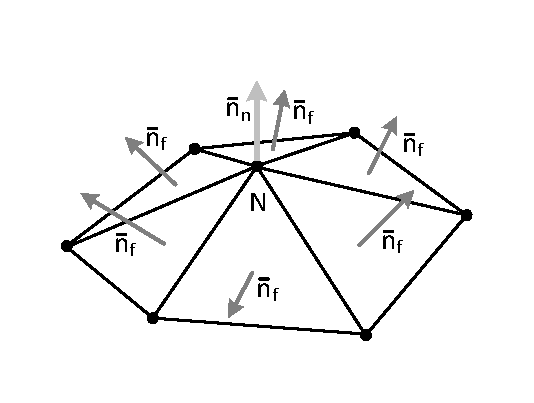
\includegraphics[width=0.4\textwidth]{pics/pic_architecture_size.pdf}
\captionstyle{center}\caption{The architecture of the computational mesh.}\label{fig:pic_architecture}
\end{figure}

The following requirements are imposed on the computational mesh.
First, the mesh must be complete, that is, each edge has exactly two incident nodes, there are no isolated and dangling nodes, and no isolated edges.
Second, all faces must be triangles (this ensures that the face is flat, since four or more arbitrary nodes may not lie in the same plane).
And thirdly, only closed meshes representing  surfaces are
considered, that is, each edge has exactly two incident faces (there
are no border edges).
\begin{equation}\label{eq_arch}
\begin{cases}
\forall N \Rightarrow \mathscr{E}(N) > 2, \mathscr{F}(N) > 2, \\
\forall e \Rightarrow \mathscr{N}(e) = 2 , \mathscr{F}(e) = 2, \\
\forall f \Rightarrow \mathscr{N}(f) = 3 , \mathscr{E}(f) = 3. \\
\end{cases}
\end{equation}
As a supplement, we will also require that the mesh is a two-sided surface, for each face the normal vector to the surface $\vec{n}_f$ is uniquely defined.
Also, no two mesh nodes are the same and there are no faces with zero area (since this would make it impossible to calculate normals).
For a mesh node, we will consider the concept of a normal to the surface and define this normal as
\begin{equation}
\vec{n}_n(N) = \frac{1}{|\mathscr{F}(N)|} \sum_{f \in
\mathscr{F}(N)}{\vec{n}_f(f)}.
\end{equation}

%---------------------------------------------------------------------------------------------------

\section{Remeshing}

The central task of rebuilding the surface due to the growth of the ice cover is as follows.
Let it be known that as a result of the numerical solution of the problem of ice formation by the finite volume method \cite{Beaugendre}, the mass of accumulated ice ($m$) was calculated in each face of the mesh.
We will assume that the density of ice is constant, that is, the volume of accumulated ice ($V$) is also known in each face.
For each mesh node $N$, it is required to find its new position $N'$ in space so that for each face with nodes $A$, $B$, $C$ the volume of space bounded by the figure $ABCA'B'C'$ corresponds to the volume of ice accumulated in this face.

It should be noted that the problem posed may not have an exact solution, in which case we should strive to minimize the volume error (when the actually formed volume of ice does not differ too much from the target volume, that is, the difference $V_{ABCA'B'C'} - V$ is relatively small).

The task of determining the new positions of the nodes of the computational mesh can be divided into two tasks: determining the directions of nodes displacements and determining the displacement values.
Next, we consider individual methods for rebuilding surfaces in more detail.

\subsection{Classical remeshing methods}

The simplest classical rebuilding methods are performed under the assumption that the direction of displacement of a node coincides with the normal drawn from this node.
Thus, it is only necessary to determine the magnitude of the offset.
Note that in the two-dimensional formulation, we can find the optimal solution (providing the minimum deviation in volume from the target value) of the problem posed \cite{Rybakov_2D}.

\begin{figure}[h]
  \centering
  \begin{minipage}[h]{0.6\textwidth}
    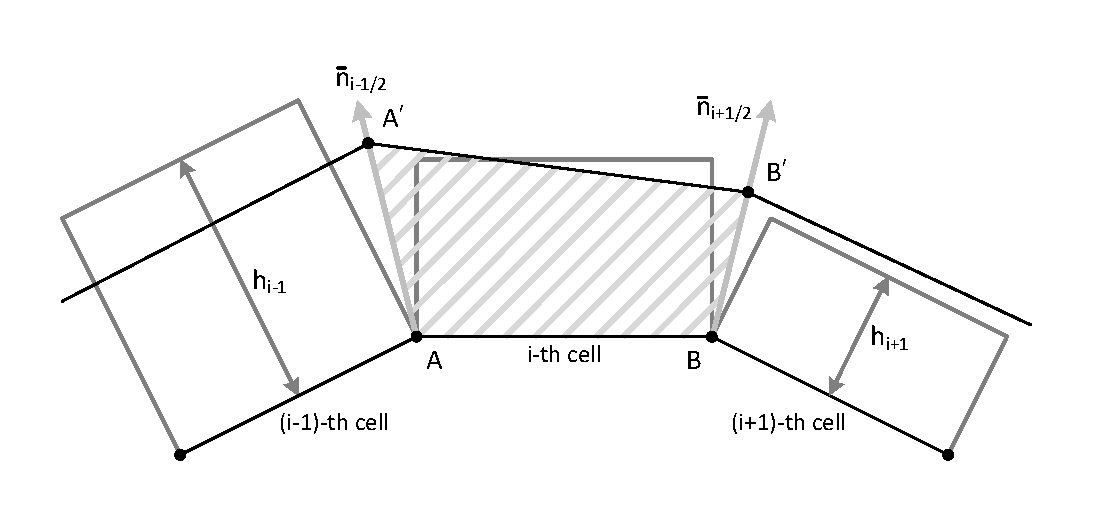
\includegraphics[width=\textwidth]{pics/pic_classical_methods_rectangles_size.pdf}
    \caption{Rebuilding the surface using the method of rectangles in 2D.}\label{fig:pic_classical_methods_rectangles}
  \end{minipage}
  \hfill
  \begin{minipage}[h]{0.6\textwidth}
    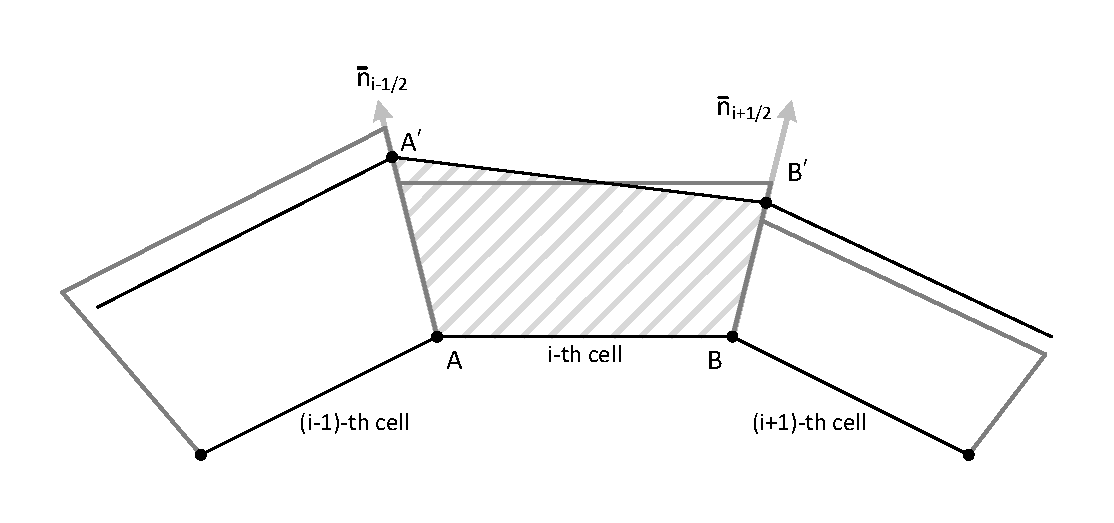
\includegraphics[width=\textwidth]{pics/pic_classical_methods_trapezoids_size.pdf}
    \caption{Surface rebuilding using the trapezoids method in 2D.}\label{fig:pic_classical_methods_trapezoids}
  \end{minipage}
\end{figure}

As the first method, let's consider the prisms method (in the two-dimensional setting, this method is analogous to the method of rectangles, shown in Fig.~\ref{fig:pic_classical_methods_rectangles}).
In this method, the input data is the amount of accumulated ice in each mesh face ($V(f)$).
At the first step, the thickness of the ice cover is searched for in each face, assuming that the ice within one face has the shape of a prism, and the face is the base of this prism.
Then, the thickness of the ice cover is equal to $h(f) =
\frac{V(f)}{S(f)}$, where $S(f)$ is the face area.
After that, the displacement value of each node is calculated simply
as the arithmetic average of the ice cover heights in all incident
faces
\begin{equation}
h(N) = \frac{1}{|\mathscr{F}(N)|} \sum_{f \in \mathscr{F}(N)}{h(f)}.
\end{equation}

The second method can be called the pyramids method (in a two-dimensional setting, this method is analogous to the trapezoids method shown in Fig.~\ref{fig:pic_classical_methods_trapezoids}).
The input data is also the volume of accumulated ice in each mesh face ($V(f)$).
However, unlike the previous method, the volume of ice accumulated in the face is represented not by a prism, but by a truncated pyramid, the base of which is the face, and the side edges are directed along the normals of the nodes.
The height of this truncated pyramid is found from the relation $V(f) = \frac{1}{3} h (2S + hS'_h + \sqrt{S(S + hS'_h)})$, where $S'_h$ is determined by the directions of the face nodes normals.
While the nodes of the face are the points of the first base of the constructed pyramid, the points of the second base are the new positions of the nodes computed relative to the considered face.
Thus, for each mesh node, several new positions are calculated (each of which is calculated relative to its incident face).
For the two-dimensional case, exactly two such new positions are obtained (since in the two-dimensional case each node has exactly two incident faces), for the three-dimensional case there are more than two such points.
To select a single new mesh node position, the average of all positions computed with respect to the incident faces is taken.

From the two methods considered, it intuitively gives the impression that the pyramids method should be more accurate, since it takes into account the loss and excess volume of ice formed due to mesh sharp fractures (since neighboring faces do not lie in the same plane, the representation of ice in faces in the form prisms inevitably leads to the formation of gaps or overlapping of ice parts in the form of prisms on top of each other).
But at least in the two-dimensional case, this assumption turns out to be wrong, since the method of rectangles shows a smaller deviation from the exact solution compared to the trapezoids method \cite{Rybakov_2D}.

\begin{figure}[h]
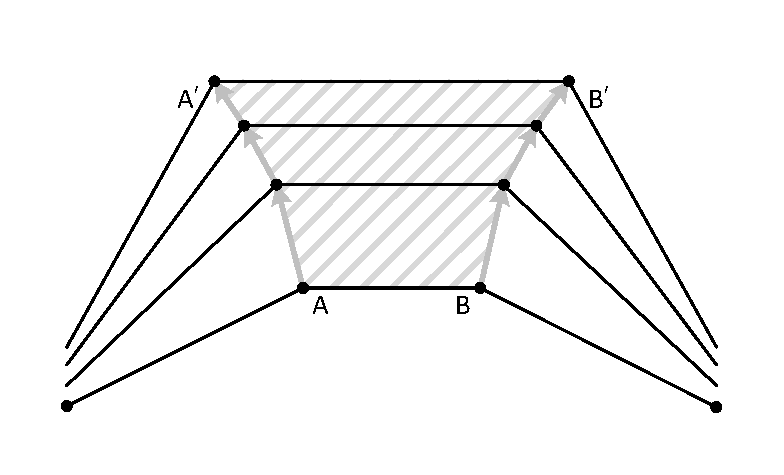
\includegraphics[width=0.48\textwidth]{pics/pic_classical_methods_multilayer_size.pdf}
\captionstyle{center}\caption{Multilayer mesh rebuilding.}\label{fig:pic_classical_methods_multilayer}
\end{figure}

Regardless of the rebuilding method used, a significant increase in accuracy can be achieved using a layered approach \cite{BourgaultCote}.
In this approach, instead of a single rebuilding of the mesh by the volume of accumulated ice in each face ($V(f)$), a fixed number of rebuilding steps $k$ is chosen, and then the procedure is performed $k$ times in a row, but using the volume of ice accumulated in the face $\frac{V(f)}{k}$.
The accuracy increases due to the fact that after each rebuilding step, the normals at the mesh nodes change their direction, and the total volume of the growing ice becomes more curvilinear, takes into account the mesh geometry better, and, as a result, more accurately corresponds to the initial value of $V(f)$ (Fig.~\ref{fig:pic_classical_methods_multilayer}).

\subsection{Rebuilding with ice volume conservation}

The articles \cite{Thompson,Tong} describe a stable iterative mesh evolution algorithm that preserves the target volume of ice.
It uses several improvements over the classical methods.

The multilayer approach implemented in this method does not use a constant number of steps -- the value of the increased volume at each step of the algorithm is calculated based on the maximum allowable fraction of the icing time step, after exceeding which numerical instability may occur in the evolution of the surface.
The most obvious case occurs when the face normal projections intersect, in which case too large time step will cause the surface to fold.
In order to  identify faces that will exhibit such behavior at the
current time step, it is assumed that the volume formed by extruding
a triangular face using a parallel displacement plane forms a
prismatoid whose volume is given by the cubic function of the height
$h$:
\begin{equation}\label{Tong:1}
V(h)=ah+bh^2+ch^3.
\end{equation}
where the constants $a$, $b$, $c$ are determined by the  positions
of the face nodes, their normals, and the face normal.
Consider the roots of the quadratic equation, which is obtained as a result of differentiation of the equation (\ref{Tong:1}).
If the roots are positive real values, the smallest positive root determines the height at which the maximum volume is reached, which is denoted as $V_{max}$, otherwise the function is monotonic with increasing and no step restriction is required in this face.
From this, it is possible to calculate the maximum fraction of the icing time step that is required to ensure reasonable volume accumulation behavior.
In addition to this step size limit, a $\alpha_{jiao}$ stability limit has been introduced.
This stability limit is based on how normal directions change as the surface evolves \cite{Jiao}.
Then, the allowable fraction of the time step for the $i$th face is
defined as
\begin{equation}\label{Tong:2}
\alpha_{\Delta t}^i=
\begin{cases}
\min(s_{\Delta t}\frac{V_{\max}^i}{V_f},\alpha_{jiao},1), \text{if $V_{\max}^i$ exists}, \\
\alpha_{jiao}, \text{if $V_{\max}^i$ doesn't exist},
\end{cases}
\end{equation}
where $s_{\Delta t}$ ($0 < s_{\Delta t} < 1$) is an  empirically
determined coefficient, $V_f$ is the current remaining ice increment
volume for the $i$th face.
Then, the volume built up for the current step is $\alpha_{\Delta t}
V_f$, where $\alpha_{\Delta t}$ is the global minimum value for all
faces.

Another important feature of the algorithm is the introduction of primary and null spaces, described in \cite{Jiao_null_space_smooth}.
If the evolutionary movement of mesh nodes occurs in primary space, then their movement in zero space will preserve the potential accuracy of the second order of the surface triangulation, so that we can maintain volume when smoothing the mesh surface.
The algorithm uses several types of smoothing.

The first smoothing is the smoothing of the normals in the mesh nodes and faces.
To make smoothing possible in zero space, all normals at nodes are calculated so that they lie in primary space, and the movement of nodes during ice buildup occurs only along their normals.
As evolution progresses, surface noise can increase, and if left unchecked, we can encounter a situation where the dihedral angle between the faces becomes too small and limits the maximum fraction of the icing time step.
To reduce surface noise, local smoothing is applied before ice builds up, adjusting the direction of node displacement in problem areas so that it more closely matches the directions of its neighbors.
This method can improve surface smoothness in some situations.
The main purpose of normal smoothing is to push points out of concave areas where normals can converge locally.
Normal smoothing is achieved using a series of weighted averages,
which are designed to give weight to the normals generated by
problem areas.

\begin{figure}[h]
  \centering
  \begin{minipage}[h]{0.49\textwidth}
    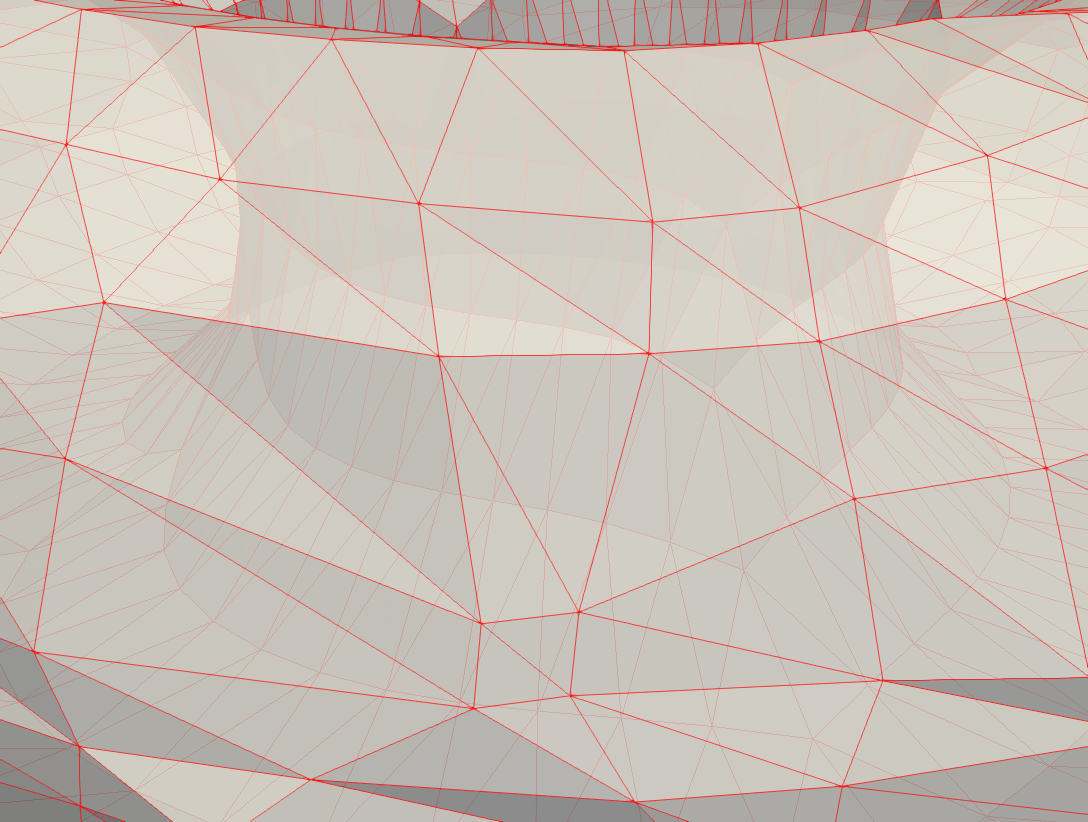
\includegraphics[width=\textwidth]{pics/pic_smooth_before.png}
    \caption{Mesh before null-space smoothing}\label{fig:pic_smooth_before}
  \end{minipage}
  \hfill
  \begin{minipage}[h]{0.49\textwidth}
    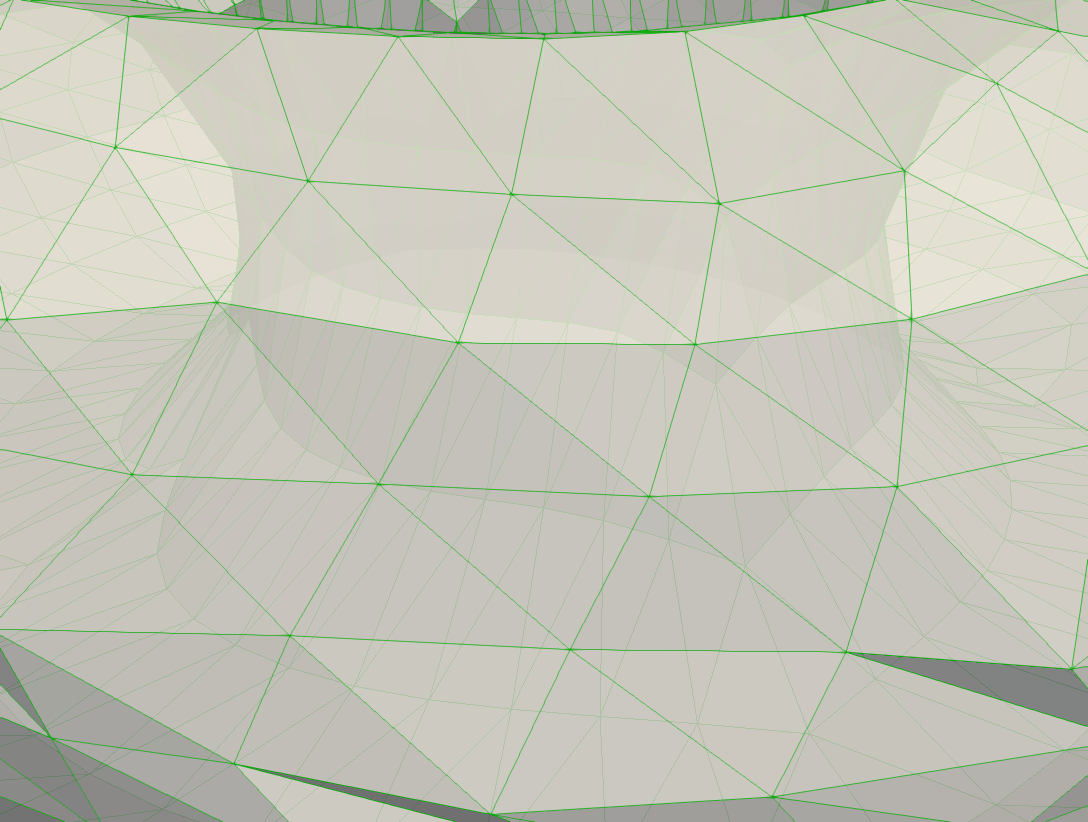
\includegraphics[width=\textwidth]{pics/pic_smooth_after.png}
    \caption{Mesh after null-space smoothing.}\label{fig:pic_smooth_after}
  \end{minipage}
\end{figure}

The second smoothing is height smoothing.
After calculating the fraction of the time step and the volume that is increased for the current step, it is necessary to determine the height field for the evolution of the surface, which will correspond to this volume, in order to determine the offsets of the mesh nodes from it.
The solution $V(h_i) = \alpha_{\Delta t} V_f$ provides the initial height field that is used to move the surface.
The purpose of the additional height smoothing step is to filter out high-frequency noise in the height field by reducing the difference in height between adjacent faces.
Usually, the heights of two triangular faces that share a common edge will not be equal.
At this step, smoothing of heights is used while preserving the volume by redistributing it between adjacent faces.

The last type of smoothing is null-space smoothing.
Surface evolution will tend to pack nodes into concave regions where surface normals converge, while mesh expansion occurs in convex regions where surface normals diverge.
If the nodes are not reallocated, it may become impossible to continue with a productive and stable time step.
To improve the quality of the surface mesh, the nodes are redistributed on the surface using null-space smoothing.
This method is able to redistribute points while maintaining the integrity of the base geometry.
Null-space is defined by a tangent plane (for smooth areas),  a
tangent line (for surface wrinkles), or empty space (for corners),
nodes moving in it remain on the surface, so that the volume and
shape of the surface can be preserved
(Figs.~\ref{fig:pic_smooth_before} and \ref{fig:pic_smooth_after}).

\subsection{Common envelope method}
Let us consider the problem of determining the new positions of the
nodes of the computational mesh in a slightly different formulation.
Let the linear rate of ice growth $v(\vec{N})$ (in meters per
second) be  known for each node $\vec{N}$.
We will assume that the growth of ice at any point of growth  is
carried out simultaneously in all directions, similar to the
Huygens--Fresnel principle of wave propagation.
Then, the ice propagation front from an arbitrary point $\vec{P}$
after a time interval $\Delta t$ will have the shape of a sphere
with center in the point $\vec{P}$ and radius $v(\vec{P}) \Delta t$.
Further, we will assume that the calculation of new positions of the nodes is performed after some fixed time $\Delta t$, that is, for each node, the radius of the ice front advance $R(\vec{N}) = v(\vec{N}) \Delta t$ is known.
Since the elements of the computational mesh are triangles, it is
necessary to determine the radius of advance of the ice front for
each internal point of the triangle according to its vertices.

Consider a computational mesh face whose vertices are the points $\vec{A}$, $\vec{B}$, $\vec{C}$.
The points of a triangle are the locus of points described as
follows
\begin{equation}
\begin{cases}
\vec{P}(\beta, \gamma) = \vec{A} + \beta (\vec{B} - \vec{A}) + \gamma (\vec{C} -
\vec{A}) = \vec{A} + \beta \vec{AB} + \gamma \vec{AC}, \\
\beta \ge 0, \quad \gamma \ge 0, \quad \beta + \gamma \le 1.
\end{cases}
\end{equation}

Let us define for each point of the triangle $\vec{P}(\beta, \gamma)$ the radius of ice front advance as $R(\vec{P}(\beta, \gamma)) = R(\beta, \gamma) = R(\vec{A}) + \beta (R(\vec{B}) - R(\vec{A})) + \gamma (R(\vec{C}) - R(\vec{A} )) = R_A + \beta R_{AB} + \gamma R_{AC}$.
The front of ice advance from the point $\vec{P}(\beta, \gamma)$ is a sphere $S(\beta, \gamma) = S(\vec{P}(\beta, \gamma), R(\beta,\gamma))$.
The ice advance front of the entire triangular face is  the common
envelope of the spheres built on all points of this face, which is
shown in Fig.~\ref{fig:pic_general_envelope_size}.

\begin{figure}
  \centering
  \begin{minipage}[b]{0.48\textwidth}
    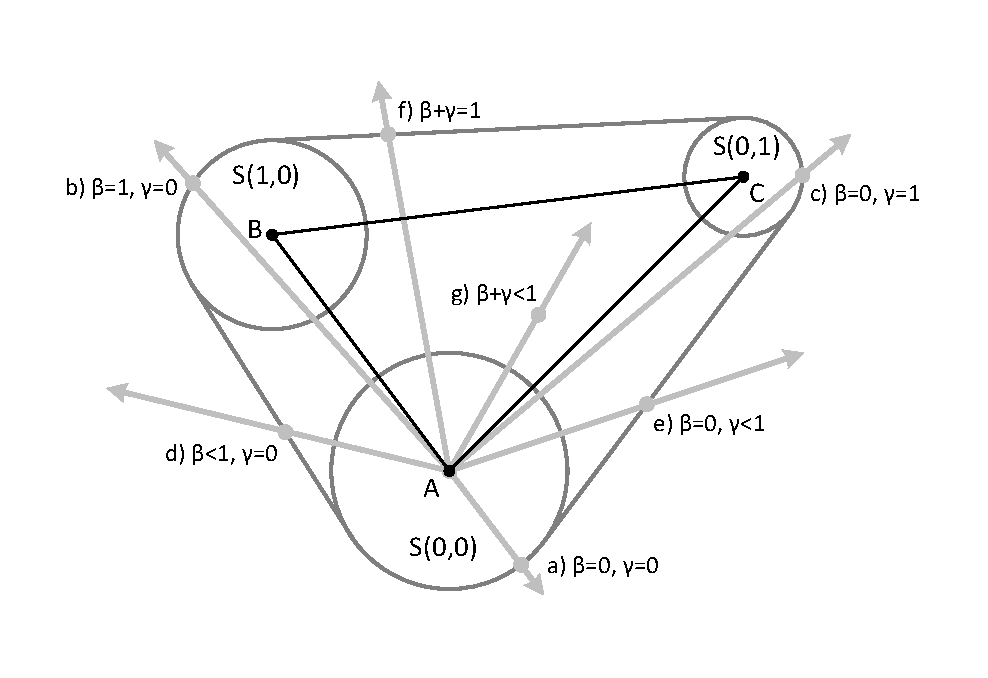
\includegraphics[width=\textwidth]{pics/pic_general_envelope_size.pdf}
    \caption{The common envelope surface of the spheres built on the points of the triangle.}\label{fig:pic_general_envelope_size}
  \end{minipage}
  \hfill
  \begin{minipage}[b]{0.48\textwidth}
    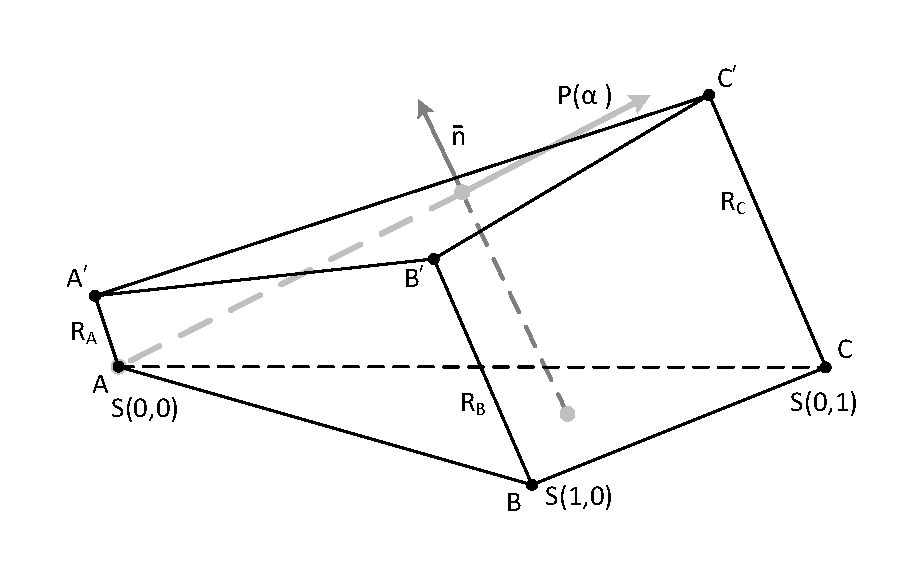
\includegraphics[width=\textwidth]{pics/pic_general_envelope_2_size.pdf}
    \caption{Finding a new node position on the common tangent plane of three spheres.}\label{fig:pic_general_envelope_2_size}
  \end{minipage}
\end{figure}

When changing the nodes positions of the computational  mesh (points
$\vec{A}$, $\vec{B}$, $\vec{C}$), we will proceed from the
assumption that after moving the nodes will be on the common
envelope surface for set of spheres $ S(\beta, \gamma)$ (new node
positions -- points $\vec{A'}$, $\vec{B'}$, $\vec{C'}$).
So far, we do not take into account the influence of neighboring
computational faces in the calculation.
Without loss of generality, we can consider only one face vertex (point $\vec{A}$).
Let the trajectory of the point $\vec{A}$ be described by the
half-line equation $\vec{P}(\alpha) = \vec{A} + \alpha \vec{D}$ for
$\alpha \ge 0$.
$\vec{D}$ is the direction vector of the point, we can assume  that
$|\vec{D}| = $1.
To find the intersection points of the trajectory of the point
$\vec{P}(\alpha) = \vec{A} + \alpha \vec{D}$ with an arbitrary
sphere $S(\beta, \gamma)$, it is necessary to substitute the
coordinates of the point $\vec{P}(\alpha)$ into the equation of the
sphere $|\vec{P} - \vec{C}(\beta, \gamma)| = R(\beta, \gamma)$,
where $\vec{C}(\beta, \gamma)$ is the center of the considered
sphere.
As a result, we get the following equation
\begin{equation}\label{eqn:intersect}
|(\vec{A} + \alpha \vec{D}) - \vec{C}(\beta, \gamma)| = R(\beta,
\gamma).
\end{equation}
This equation must be solved for the unknown $\alpha$ with fixed parameters $\beta$ and $\gamma$.
This equation is quadratic, it has no more than two roots, which depend on the parameters $\alpha_{1,2} = \alpha_{1,2}(\beta, \gamma)$.
To determine the new position of the point $\vec{A}$, it is necessary to find the maximum value of the real root of such an equation for all admissible values of the parameters.
In this case, the intersection point of the trajectory of the
movement of the point  $\vec{A}$ with the common envelope of the
family of spheres can be located in different parts of this
envelope, which is shown in Fig.~\ref{fig:pic_general_envelope_size}
and is associated with the conditions that the parameters $\beta$
and $\gamma$ (points a), b), c) -- intersection with a sphere with
center in the triangle vertices, points d), e), f) -- intersection
with a sphere with center on the triangle edges, point g) --
intersection with the sphere centered inside the triangle).

The equation (\ref{eqn:intersect}) can be written as $|\alpha
\vec{D} -  (\beta \vec{AB} + \gamma \vec{AC})|^2 = (R_A + \beta
R_{AB} + \gamma R_{AC})^2$ or explicitly as a quadratic equation
\begin{equation}
|\vec{D}|^2 \alpha^2 - 2(\beta (\vec{D}, \vec{AB}) +  \gamma
(\vec{D}, \vec{AC})) \alpha + |\beta \vec{AB} + \gamma \vec{AC}|^2 -
(R_A + \beta R_{AB} + \gamma R_{AC})^2 = 0
\end{equation}
The largest root of this equation (taking into account the condition
$|\vec{D}| = 1$) can be written explicitly
\begin{multline}
\alpha(\beta, \gamma) = \beta (\vec{D}, \vec{AB}) + \gamma (\vec{D}, \vec{AC}) \\
+\sqrt{(\beta (\vec{D}, \vec{AB}) + \gamma (\vec{D}, \vec{AC}))^2 -
|\beta \vec{AB} + \gamma \vec{AC}|^2 + (R_A + \beta R_{AB} + \gamma
R_{AC})^2}
\end{multline}
or
\begin{equation}
\begin{cases}
\alpha(\beta, \gamma) = k_{\beta} \beta + k_{\gamma} \gamma + \sqrt{T}, \\
T = q_{\beta^2} \beta^2 + q_{\gamma^2} \gamma^2 + q_{\beta \gamma} \beta \gamma + q_{\beta} \beta + q_{\gamma}
\gamma + q, \\
k_{\beta} = (\vec{D}, \vec{AB}), k_{\gamma} = (\vec{D}, \vec{AC}), \\
q_{\beta^2} = (\vec{D}, \vec{AB})^2 - |\vec{AB}|^2 + R_{AB}^2, q_{\gamma^2} = (\vec{D}, \vec{AC})^2 -
|\vec{AC}|^2 + R_{AC}^2, \\
q_{\beta \gamma} = 2 ((\vec{D}, \vec{AB})(\vec{D}, \vec{AC}) - (\vec{AB}, \vec{AC}) + R_{AB} R_{AC}), \\
q_{\beta} = 2 R_A R_{AB}, q_{\gamma} = 2 R_A R_{AC}, q = R_A^2.
\end{cases}
\end{equation}
To search for a new position of the point $\vec{A}$, it is required
to find the maximum of the expression $\alpha(\beta, \gamma)$
subject to the constraints $\beta \ge 0$, $\gamma \ge 0$, $\beta +
\gamma \le 1$.
The maximum of the expression $\alpha(\beta, \gamma)$ is achieved
either when the center of the sphere is inside the triangle or on
one of its sides.

If the center of the sphere is on side $AB$ of triangle  $ABC$, the
condition $\gamma = 0$ is satisfied, and the expression for $\alpha$
is $\alpha_{\gamma = 0}(\beta) = k_{\beta} \beta + \sqrt{q_{\beta^2}
\beta^2 + q_{\beta} \beta + q}$.
If the center of the sphere is on side $AC$ of triangle $ABC$,  the
condition $\beta = 0$ is satisfied, and the expression for $\alpha$
is $\alpha_{\beta = 0}(\gamma) = k_{\gamma} \gamma +
\sqrt{q_{\gamma^2} \gamma^2 + q_{\gamma} \gamma + q}$.
If the center of the sphere is on side $BC$ of triangle $ABC$,  the
condition $\beta + \gamma = 1$ is satisfied, and the expression for
$\alpha$ takes the following form
\begin{multline}
\alpha_{\beta + \gamma = 1}(\gamma) = (k_{\gamma} - k_{\beta}) \gamma + k_{\beta}  \\
+\sqrt{(q_{\beta^2} + q_{\gamma^2} - q_{\beta \gamma}) \gamma^2 +
(-2 q_{\beta^2} + q_{\beta \gamma} - q_{\beta} + q_{\gamma}) \gamma
+ (q_{\beta^2} + q_{\beta} + q)}.
\end{multline}
In all cases, where the center is on one of the triangle sides, the
problem of finding the maximum value of $\alpha(\beta, \gamma)$
under given constraints is reduced to the problem of finding the
maximum value of a function which has a form $\alpha(x) = k_x x + k
+ \sqrt {q_{x^2} x^2 + q_x x + q}$ (taking into account these
restrictions), which is not difficult (the maximum point is either a
local extremum point or a boundary point of the function's domain).

We should separately consider the option in which the center of  the
desired sphere is inside the triangle.
In this case, the intersection point of the trajectory
$\vec{P}(\alpha) = \vec{A} + \alpha \vec{D}$ with the common
envelope is on the common tangent plane to the spheres $S(0, 0)$,
$S(1, 0)$, $S(0, 1)$ (plane $A'B'C'$, see
Fig.~\ref{fig:pic_general_envelope_2_size}).

The center of the desired sphere is found at the intersection  point
of the plane $ABC$ and the straight line passing through the point
$\vec{P}(\alpha)$ and directed along the normal to the plane
$A'B'C'$.
If the vector of the unit normal of the plane $A'B'C'$ is  denoted
by $\vec{n}$, then the relationship between the points of the planes
$ABC$ and $A'B'C'$ can be expressed as follows
\begin{equation}
\begin{cases}
\vec{A'} = \vec{A} + \vec{n} R_A, \\
\vec{B'} = \vec{B} + \vec{n} R_B, \\
\vec{C'} = \vec{C} + \vec{n} R_C.
\end{cases}
\end{equation}

To find the vector $\vec{n}$, we use the fact that  the result of
the vector product $\vec{A'B'} \times \vec{A'C'}$ is collinear to
the vector $\vec{n}$.
Let's write it explicitly
\begin{equation}
(\vec{AB} + \vec{n} R_{AB}) \times (\vec{AC} + \vec{n} R_{AC}) = t
\vec{n},
\end{equation}
\begin{equation}
\vec{AB} \times \vec{AC} + R_{AB} (\vec{n} \times \vec{AC}) - R_{AC}
(\vec{n} \times \vec{AB}) = t \vec{n},
\end{equation}
\begin{equation}
t
\left[ { \begin{array}{c}
            n_x \\
            n_y \\
            n_z \\
         \end{array} } \right]
+ R_{AC}
\left[ { \begin{array}{c}
            n_y AB_z - n_z AB_y  \\
            n_z AB_x - n_x AB_z \\
            n_x AB_y - n_y AB_x \\
         \end{array} } \right]
- R_{AB}
\left[ { \begin{array}{c}
            n_y AC_z - n_z AC_y \\
            n_z AC_x - n_x AC_z \\
            n_x AC_y - n_y AC_x \\
         \end{array} } \right]
= \vec{AB} \times \vec{AC}.
\end{equation}

This relation can be satisfied for $t > 0$, or for  $t < 0$, which
corresponds to the existence of two common tangent planes to three
spheres.
Let us rewrite the above relation as a system  of linear equations
with respect to the components of the normal for an arbitrary value
of the parameter $t$:
\begin{equation}
\left[ { \begin{array}{ccc}
             t & R_{AC} AB_z - R_{AB} AC_z & R_{AB} AC_y - R_{AC} AB_y \\
             R_{AB} AC_z - R_{AC} AB_z & t & R_{AC} AB_x - R_{AB} AC_x \\
             R_{AC} AB_y - R_{AB} AC_y & R_{AB} AC_x - R_{AC} AB_x & t \\
         \end{array} } \right]
\left[ { \begin{array}{c}
            n_x \\
            n_y \\
            n_z \\
         \end{array} } \right]
= \vec{AB} \times \vec{AC}.
\end{equation}
From this system of equations, two possible directions of the normal
to the common tangent plane of the spheres $S(0,0)$, $S(1,0)$, $S(0,
1)$ are found.
For each direction of the normal, the plane $A'B'C'$ and the point $\vec{P}(\alpha) = \vec{A} + \alpha \vec{D}$ on it (and the required parameter $\alpha$) are found.
This point can be taken into account in the general set of solutions only if it corresponds to the sphere $S(\beta, \gamma)$, whose parameters satisfy the three conditions $\beta \ge 0$, $\gamma \ge 0$, $ \beta + \gamma \le 1$.
The parameters $\beta$ and $\gamma$ can be determined by finding the intersection point of the line $\vec{P}(\alpha) - x \vec{n}$, $x \in \mathbb{R}$ and the plane $ABC$.

Thus, having found solutions to all potentially possible special
cases presented in Fig.~\ref{fig:pic_general_envelope_size}, we find
a set of solutions $\alpha$, from which, to determine the actual new
position of the point $A'$, it is necessary to take the maximum one.

The above algorithm concerns the obtaining of the node offset given only one incident face.
When considering a separate mesh node, it is required to calculate the displacement of this node relative to each incident face and choose the maximum among these displacements.

\begin{figure}[h]
  \centering
  \begin{minipage}[h]{0.55\textwidth}
    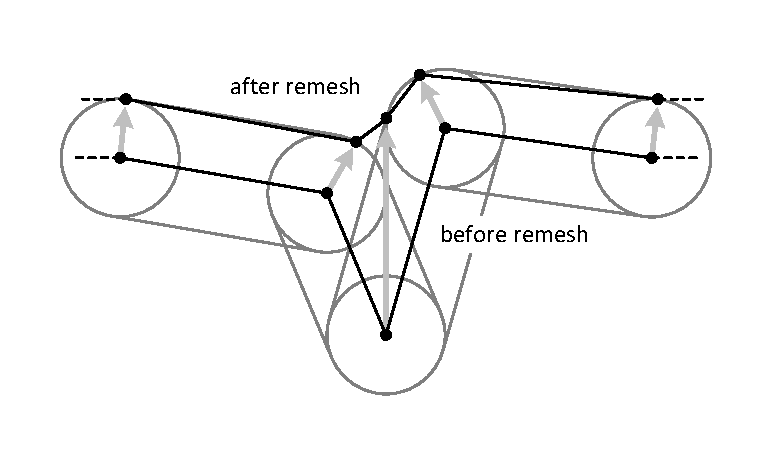
\includegraphics[width=\textwidth]{pics/pic_general_envelope_3_size.pdf}
    \caption{Example of tightening of a cavity in a 2D diagram.}\label{fig:pic_general_envelope_3_size}
  \end{minipage}
  \hfill
  \begin{minipage}[h]{0.44\textwidth}
    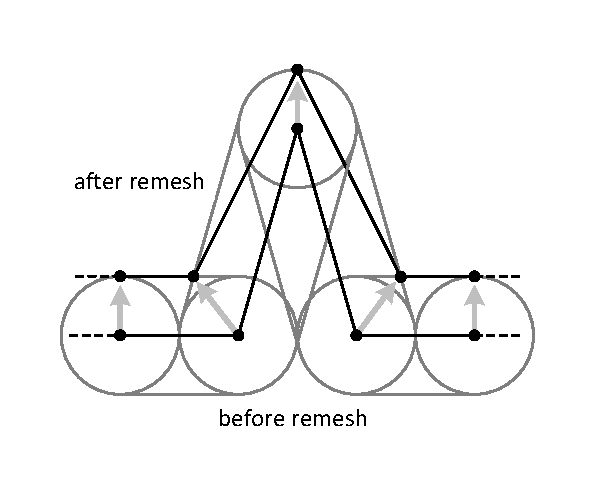
\includegraphics[width=\textwidth]{pics/pic_general_envelope_4_size.pdf}
    \caption{Example of smoothing a sharp peak in a 2D diagram.}\label{fig:pic_general_envelope_4_size}
  \end{minipage}
\end{figure}

\begin{figure}[h]
  \centering
  \begin{minipage}[h]{0.49\textwidth}
    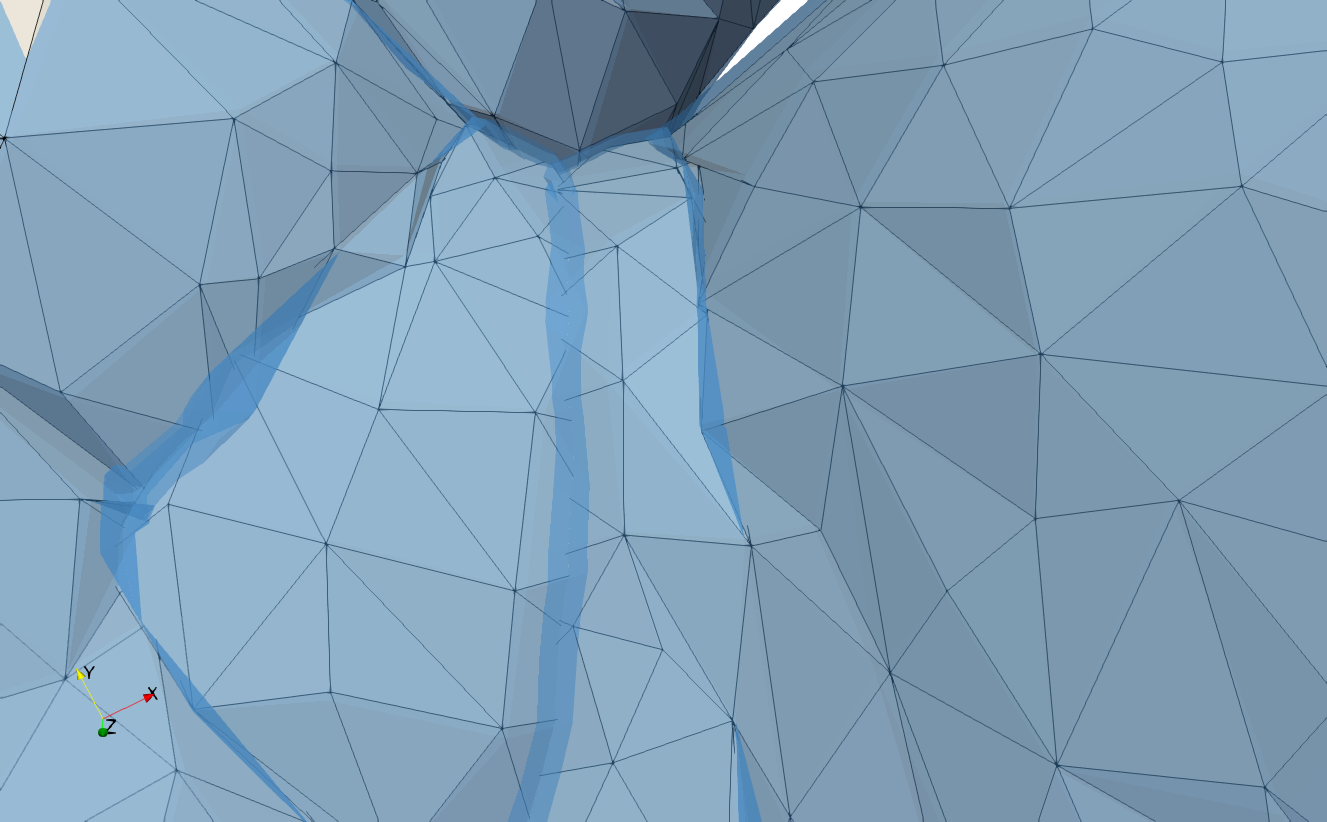
\includegraphics[width=\textwidth]{pics/pic_envelope_cave.png}
    \caption{Example of tightening for a 3D surface.}\label{fig:pic_general_envelope_cave}
  \end{minipage}
  \hfill
  \begin{minipage}[h]{0.49\textwidth}
    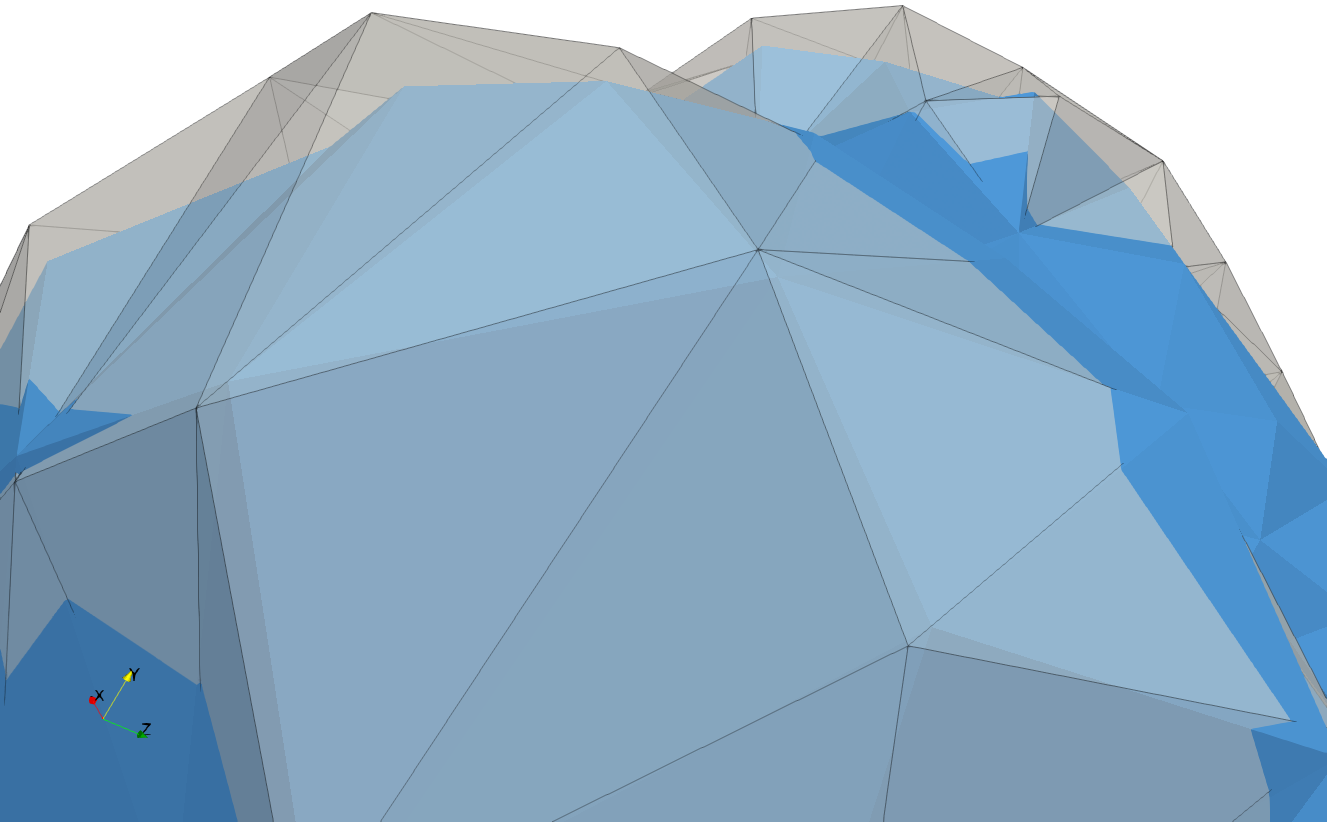
\includegraphics[width=\textwidth]{pics/pic_envelope_peak.png}
    \caption{Example of smoothing sharp peaks for a 3D surface.}\label{fig:pic_envelope_peak}
  \end{minipage}
\end{figure}

The algorithm for determining the new positions of nodes from the common envelope for family of spheres is linear in the number of nodes (we assume that on meshes suitable for calculations, the number of incident faces for one node is limited by a reasonable number) and does not contain iterative procedures.
The algorithm has the peculiarity of tightening small depressions and noise on the mesh.
This is due to the fact that the node $\vec{N}$, being at the bottom of the cavity, has the ability to move in the direction of exit from this cavity to a distance greater than $R(\vec{N})$, which is shown in Fig.~\ref{fig:pic_general_envelope_3_size}.
Another interesting feature is the operation of the algorithm on mesh areas with sharp peaks (Fig.~\ref{fig:pic_general_envelope_4_size}).
It can be seen from this figure that during the operation of the algorithm, sharp peaks tend to smooth out.
Thus, the new node positions form a smoother surface than it was before the rebuild.

Figure~\ref{fig:pic_general_envelope_cave} demonstrates the effect
of cavity tightening compared to the classical prisms method (cavity
tightening is marked in blue on the mesh).
Figure~\ref{fig:pic_envelope_peak} shows the opposite effect --
smoothing of sharp peaks (compared to the same classical prisms
method).

%---------------------------------------------------------------------------------------------------

\section{Adaptation}

All methods of rebuilding surfaces considered in the previous section have one thing in common -- they preserve the number of elements of the computational mesh (nodes, edges, faces) and the connections between them.
Despite some special methods for preventing collisions between mesh faces and smoothing methods, after the formation of a new surface, self-intersections, irregularly shaped faces, and uneven distribution of faces in the mesh in size can occur.
For the time being, we will omit the self-intersections of the mesh and consider only questions concerning the shape and size of the faces.

\begin{figure}[h]
  \centering
  \begin{minipage}[h]{0.35\textwidth}
    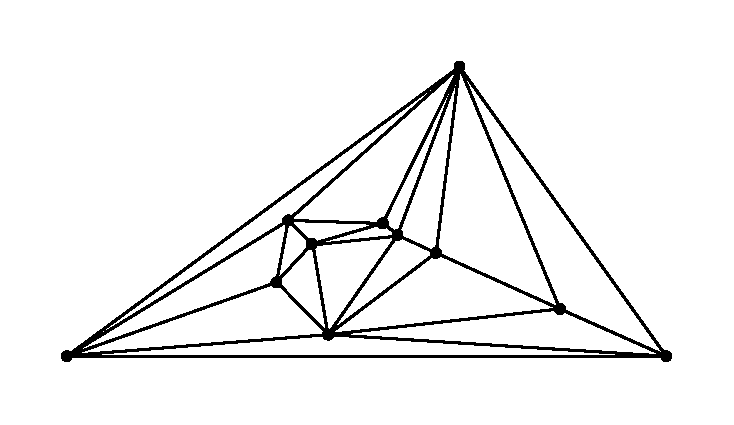
\includegraphics[width=\textwidth]{pics/pic_delaunay_size.pdf}
    \caption{Splitting a face using Delaunay triangulation.}\label{fig:pic_delaunay}
  \end{minipage}
  \hfill
  \begin{minipage}[h]{0.35\textwidth}
    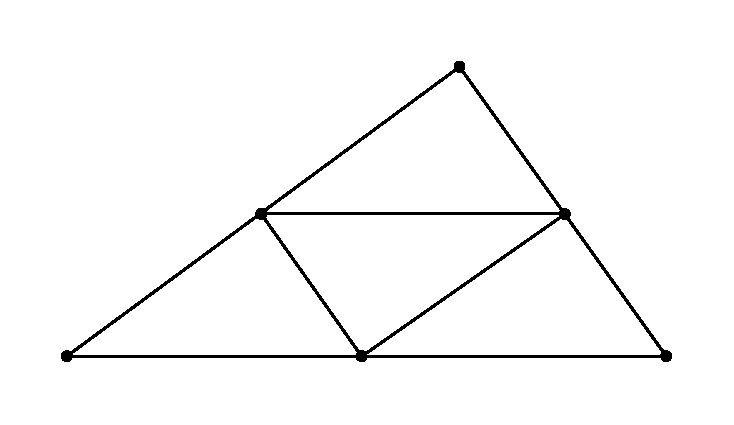
\includegraphics[width=\textwidth]{pics/pic_delaunay_2_size.pdf}
    \caption{Breaking up a face into smaller ones.}\label{fig:pic_delaunay_2}
  \end{minipage}
  \hfill
  \begin{minipage}[h]{0.28\textwidth}
    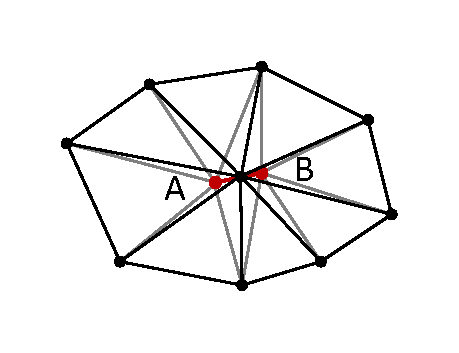
\includegraphics[width=\textwidth]{pics/pic_reduce_edge_size.pdf}
    \caption{Edge reducing.}\label{fig:pic_reduce_edge}
  \end{minipage}
\end{figure}

The first operation that we need is to split the face into smaller ones.
In all cases, we will split the faces using Delaunay triangulation, assuming that we know a set of points inside the face and we have to split the face using them (Fig.~\ref{fig:pic_delaunay}) \cite{Rivara}.
It is worth noting that face partitioning can be performed while preserving the local curvature of the mesh, as shown in \cite{Rakotoarivelo}, but for simplicity, we will partition only in the face plane.
If the split point is located not inside the face, but on its edge, then the second incident face of this edge will also have to be split (only meshes are considered whose edges have exactly two incident faces, as indicated in (\ref{eq_arch}).
Sometimes, to reduce the size, it is simply needed to split the face into smaller ones without setting split points.
In this case, it is necessary to monitor the quality of the resulting faces.
To determine the shape quality of a triangular face with nodes
$\vec{A}$, $\vec{B}$, $\vec{C}$, we can use a simple quality
criterion
\begin{equation}
Q(f) = \frac{4\sqrt{3} S_{ABC}}{|\vec{AB}|^2 + |\vec{BC}|^2 +
|\vec{AC}|^2},
\end{equation}
where $Q(f) = 1$ corresponds to the ideal case of an equilateral
face, and $Q(f) = 0$ is the worst case for faces with zero area
\cite{Borouchaki}.
To split a face into smaller ones while maintaining their quality, simply perform a split in the middle of all its sides (Fig.~\ref{fig:pic_delaunay_2}).

The second operation, which is necessary for mesh adaptation, is related to coarsening.
Quite often, when performing triangulation over a set of given points, faces with a low quality indicator may appear (they may have either too sharp corners or a corner close to $2 \pi$).
If the face contains an angle close to $2 \pi$, then splitting along the largest side will help to get rid of it (in this case, the base of the height lowered from the opposite node should be chosen as the splitting point).
If the triangle contains only close to acute angles, then it has a side that is too short, which can be removed.
When an edge $AB$ is removed, both faces incident to it are removed, nodes $A$ and $B$ are connected into a single node $A'$, and all edges from the set $\mathscr{E}(A) \cup \mathscr{E} (B)$ are redirected to node $A'$, taking into account the removal of doubles (Fig.~\ref{fig:pic_reduce_edge}).
This operation will be called edge reducing \cite{Panchal}.
By applying the reducing of the shortest edges in the  computational
mesh, we can achieve an arbitrary degree of coarsening.

%---------------------------------------------------------------------------------------------------

\section{Self-intersections elimination}

The main problem that can potentially be encountered in the evolution of the computational mesh is the occurrence of self-intersections.
Self-intersection is a critical mesh defect, which makes it impossible to perform further calculations on ice formation modeling, so self-intersections must be removed.
First, it is necessary to determine what ratio of two mesh faces can be interpreted as self-intersection.
Of course, the mere presence of common points in two faces cannot serve as a criterion for self-intersection, since each face has adjacent faces (that is, two faces can have both a common vertex and a common edge).
Since only faces that have common incident objects  (a common
incident vertex or a common incident edge) can be adjacent, and all
incidence relations are written in the computational mesh, it is not
difficult to separate the intersection of faces by a common incident
object from self-intersection.

\subsection{Search for pairs of intersecting triangles}

In any case, to identify all facts of mesh self-intersection, it is required to analyze all pairs of faces and check the intersection of faces in the pair (that is, check the intersection of each face with each).
Since direct enumeration of all faces pairs has quadratic complexity in terms of the number of faces in the mesh, so direct approach for large meshes is impossible.
In this case, it is advisable to search for pairs of intersecting faces using the representation of a set of faces in the form of a special tree structure associated with boxing of geometric objects by rectangular parallelepipeds in space.
First, let's define the concept of a container for an  arbitrary set
of points $M$ in space (we will denote it by $[M]$): $[M]$ is a
rectangular parallelepiped that is the Cartesian product of three
segments
\begin{equation}
[M] = \left[\min_{P \in M}{P_x}, \max_{P \in M}{P_x}\right]
      \times \left[\min_{P \in M}{P_y}, \max_{P \in M}{P_y}\right]
      \times \left[\min_{P \in M}{P_z}, \max_{P \in M}{P_z}\right].
\end{equation}

The container can be considered for an arbitrary set of points.
We will use it for a face of the computational mesh, as well as for a set of faces.
Since any triangle is a convex figure, then $[ABC] = [\{A, B, C\}]$, that is, to construct a container for a triangle, it is enough to consider only its vertices.
When searching for pairs of intersecting faces, we will use the following fact: if two triangles intersect, then their containers also intersect: $ABC \cap A'B'C' \ne \emptyset \Rightarrow [ABC] \cap [A'B'C'] \ne\emptyset$.
This means that if the containers of two triangles do not
intersect, then the triangles themselves do not intersect: $[ABC]
\cap [A'B'C'] = \emptyset \Rightarrow ABC \cap A'B'C' = \emptyset$.
Unlike the analysis of a pair of triangles for intersection,
checking for  the intersection of two rectangular boxes with sides
parallel to the coordinate axes is not a problem.
That is, at the first stage, we will look for such pairs of faces
whose  containers intersect (we will call them potentially
intersecting faces).

\begin{figure}[h]
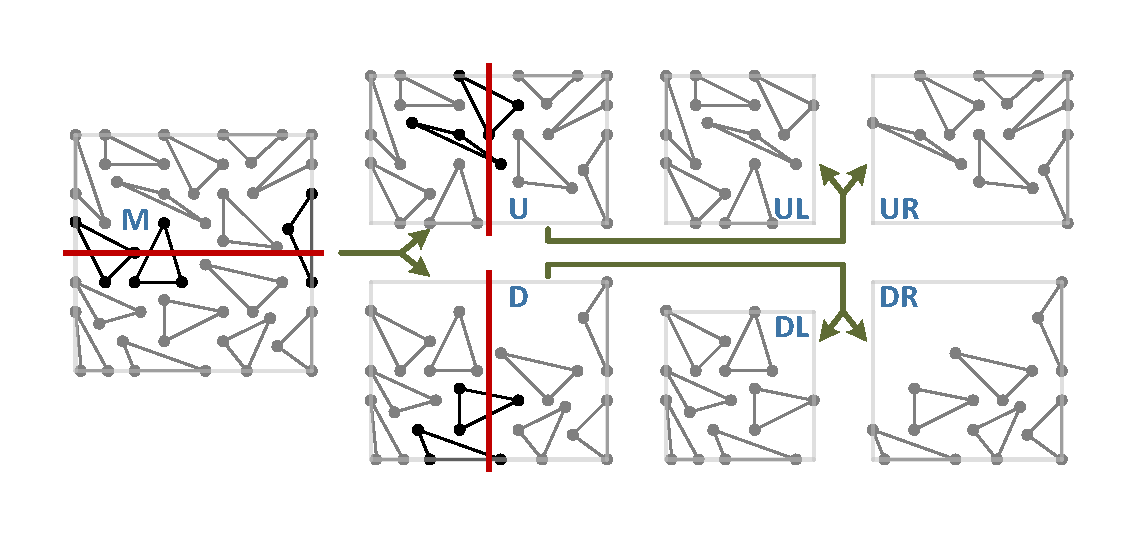
\includegraphics[width=0.8\textwidth]{pics/pic_box_size.pdf}
\captionstyle{center}\caption{Scheme for building a container tree.}\label{fig:pic_box}
\end{figure}

To search for potentially intersecting faces, we build a tree of
containers  for all mesh faces.
The root of this tree will be the container of all faces of the
computational  mesh.
Consider the procedure for dividing a container into two smaller
containers  using the two-dimensional case illustrated in
Fig.~\ref{fig:pic_box} as an example.
We want to divide the container of some set of triangles ($M$) along
a  horizontal straight line into two sets: upper set ($U$ -- up) and
lower set ($D$ -- down).
Then, all triangles that lie above the line or intersect it will
fall into the upper set.
Similarly, all triangles that lie below the line or intersect it will fall into the lower set.
After selecting the upper and lower sets of triangles, for each of them their own containers are built, which become child containers of the original one.
After that, the resulting containers can be divided further using an arbitrary splitting direction ($X$, $Y$, $Z$).
In particular, Fig.~\ref{fig:pic_box} demonstrates the splitting of the original container according to the scheme $[M] \rightarrow \{[U], [D]\} \rightarrow \{\{[UL], [UR]\}, \{[DL], [DR]\}\}$.
It should be noted that in one operation, a container can be split into an arbitrary number of child containers in a similar way.
As the direction of splitting the container, it is advisable to choose the most extended one (along which the length of the container has the greatest value).

The constructed container tree makes it possible to significantly reduce the number of tested potential intersections of triangles \cite{Jung}, since if $[M] \cap [M'] = \emptyset$, $[T]$ is a child container for $[M]$ , and $[T']$ is a child container for $[M']$, then $[T] \cap [T'] = \emptyset$.

After all pairs of potentially intersecting triangles have been found, it is necessary to check whether they actually intersect.
Since a triangle is a convex figure, the intersection of two triangles is also a convex figure (it can be any flat figure with 1 to 6 vertices).
The vertices of the intersection of two triangles are the points of intersection of the sides of one triangle with another triangle and vice versa.
Thus, the problem of finding the intersection of two triangles is reduced to finding the intersection points of a triangle and a segment.
This problem can be solved by representing triangle $ABC$ as a locus of points $\vec{P} = \vec{A} + \beta \vec{AB} + \gamma \vec{AC}$, $\beta \ge 0$, $\gamma \ge 0$, $\beta + \gamma \le 1$, representations of the segment $QR$ as the locus of points $\vec{P} = \vec{Q} + \phi \vec{QR}$, $0 \le \phi \le 1$ and finding a solution to the system of equations $\vec{A} + \beta \vec{AB} + \gamma \vec{AC} = \vec{Q} + \phi \vec{QR}$ with respect to the unknowns $\beta$, $\gamma$, $\phi$ subject to constraints \cite{Freylekhman}.

\subsection{Fixing intersecting triangles}

After all pairs of intersecting faces and areas of their intersections are found, it is necessary to determine a strategy for their elimination.
All faces of the computational mesh can be divided into three categories.
The first category is faces that do not intersect with any other faces, and which should become part of the final surface (we will assume that at any time we have the opportunity to specify an arbitrary number of such faces).
We will call such faces static.
The second category is faces that do not intersect with any other faces, but that should not become part of the final surface (faces of internal self-intersection loops of the surface that must be removed).
We will call such faces hidden.
The third category is faces that intersect with some other faces.
Such faces will be called intersection faces.

\begin{figure}[h]
  \centering
  \begin{minipage}[h]{0.3\textwidth}
    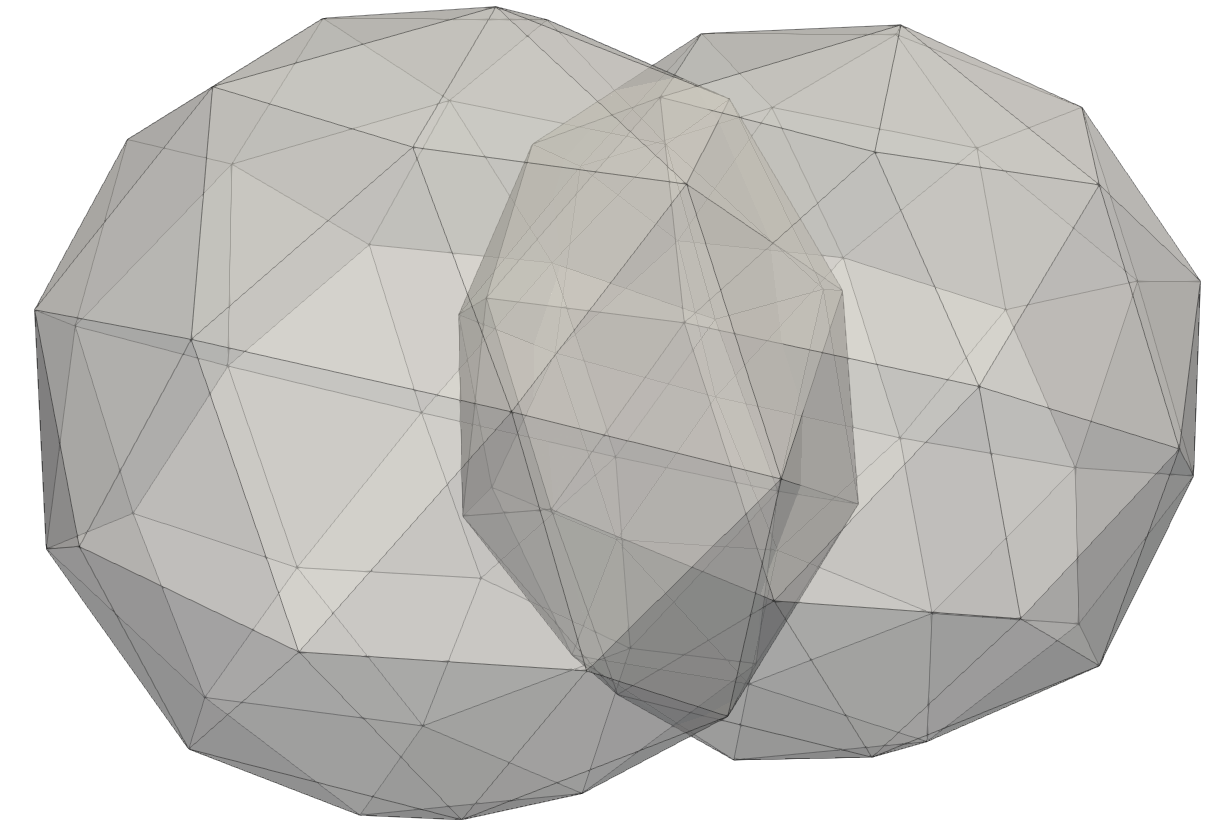
\includegraphics[width=\textwidth]{pics/pic_zip_01.png}
    \caption{Intersection of computational meshes for two spheres.}\label{fig:pic_zip_01}
  \end{minipage}
  \begin{minipage}[h]{0.3\textwidth}
    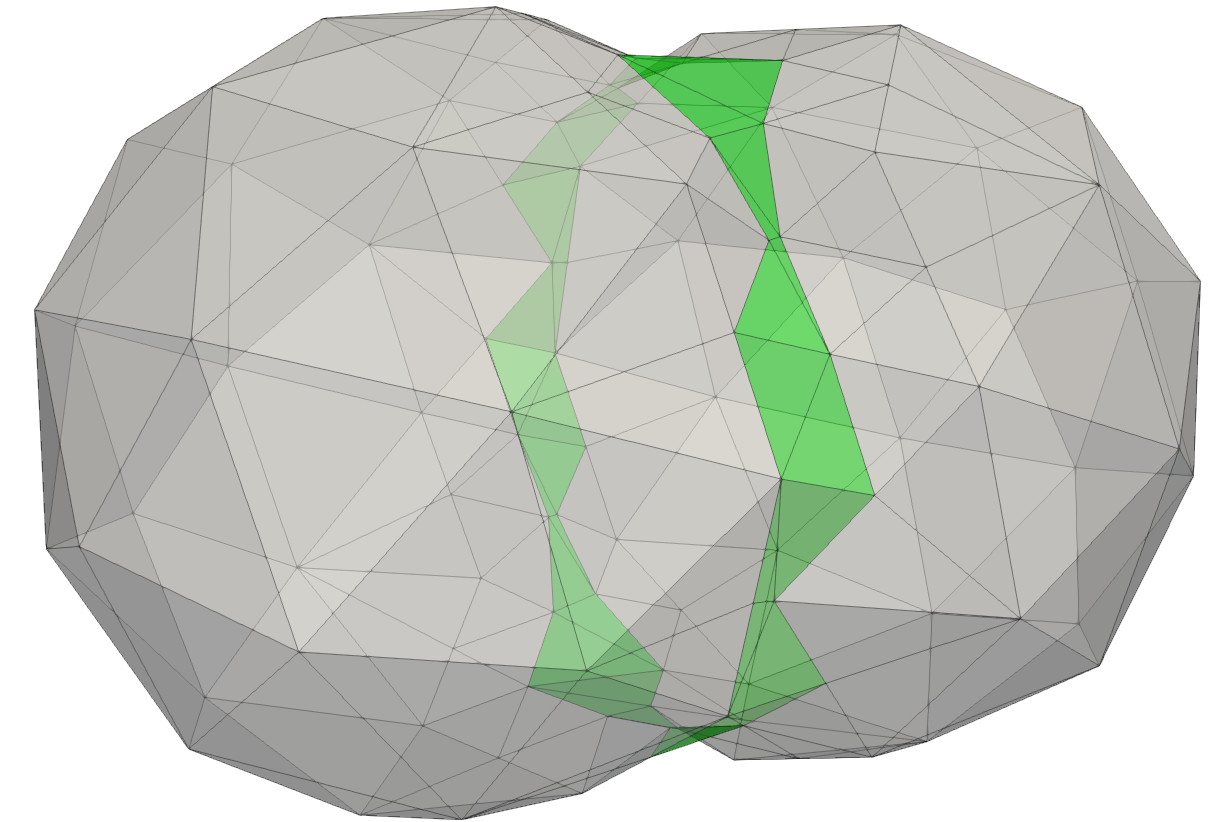
\includegraphics[width=\textwidth]{pics/pic_zip_09.png}
    \caption{Rough removal of intersection faces.}\label{fig:pic_zip_09}
  \end{minipage}
  \begin{minipage}[h]{0.3\textwidth}
    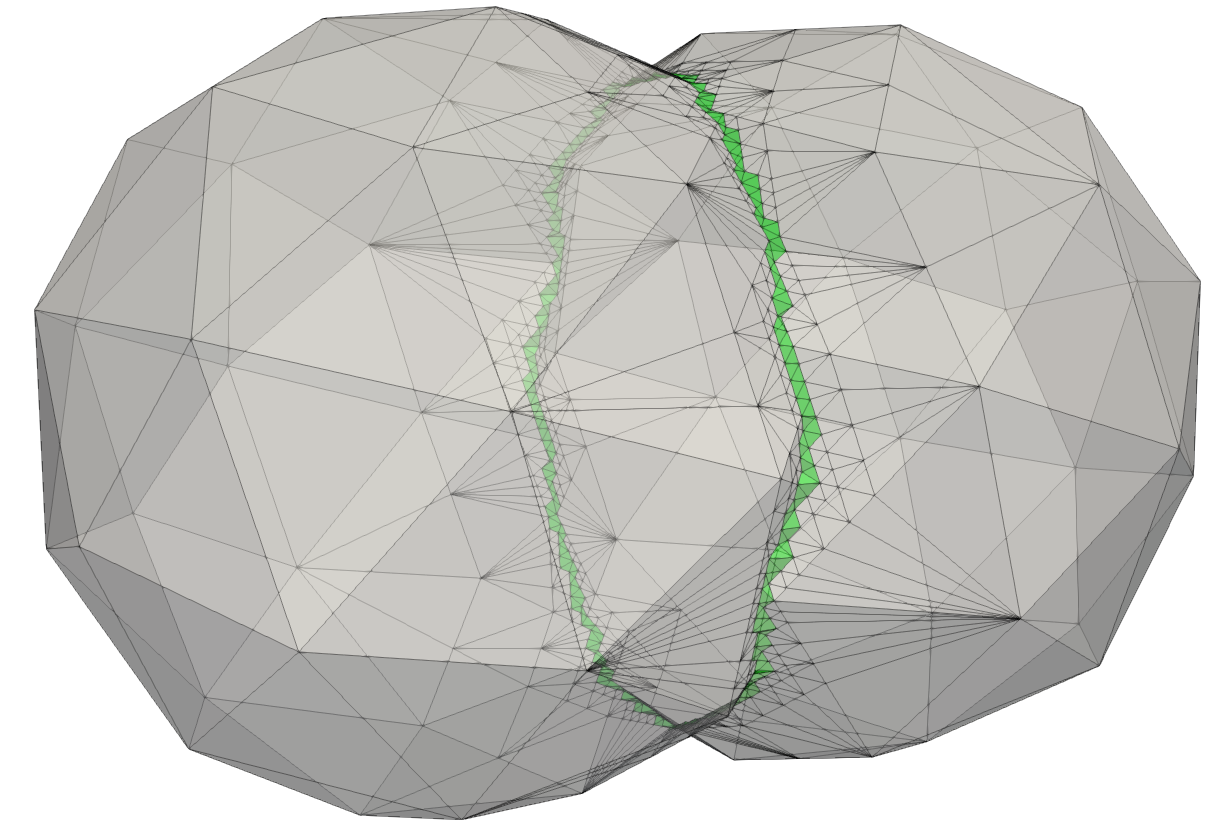
\includegraphics[width=\textwidth]{pics/pic_zip_15.png}
    \caption{Removing intersection faces after splitting.}\label{fig:pic_zip_15}
  \end{minipage}
\end{figure}

One approach to eliminating mesh self-intersections is to simply remove all intersection faces.
After performing this operation, the mesh is divided into areas of static and hidden faces.
In this case, the hidden faces are unreachable from the static areas when the faces of the computational mesh are bypassed (if only the faces adjacent along the edge are considered neighbors during the bypass).
After the hidden faces are removed from the mesh, the computational mesh consists only of static faces, but some new faces must be added to restore the integrity of the mesh \cite{Charton}.
This approach to eliminating mesh self-intersections can be used for relatively simple surfaces, but in general it does not guarantee a correct result.
As an illustration of such a way to eliminate intersections,
Figs.~\ref{fig:pic_zip_01} and~\ref{fig:pic_zip_09} shows an example
of work to eliminate intersections of the computational meshes of
two spheres (new faces that appear when the mesh is restored are
marked in green).
In Fig.~\ref{fig:pic_zip_09} we can note the rather low quality of the resulting mesh.
It is possible to improve the quality by splitting the intersection faces.
That is, after searching for all intersection faces, they must be split into smaller ones (as shown in Fig.~\ref{fig:pic_delaunay_2}), then repeat the procedure for deleting intersection faces and hidden faces and finally restore the mesh.
The process of splitting the intersection faces can be repeated many times, while the quality of the resulting mesh will increase, as shown in Fig.~\ref{fig:pic_zip_15}.

With another approach to eliminate self-intersections, no faces are removed from the mesh, but are split into smaller ones at all intersection points \cite{Skvorkovska}.
As an example, Fig.~\ref{fig:pic_before_cut} shows two triangles that intersect along a segment (two points of intersection).
After splitting, we get the construction shown in Fig.~\ref{fig:pic_after_cut}.
In the general case, there can be an arbitrarily large number of points at which it is necessary to split a face, and splitting should be performed by triangulating over these points, and some edges of the triangulation should be predefined.

\begin{figure}[h]
  \centering
  \begin{minipage}[h]{0.38\textwidth}
    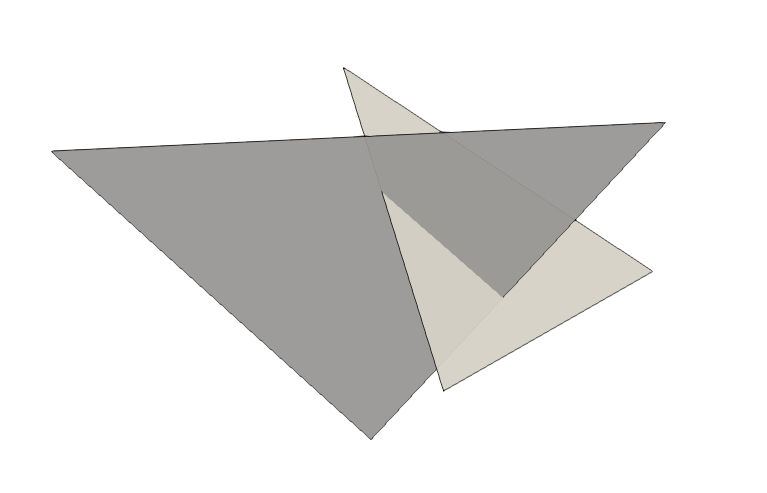
\includegraphics[width=\textwidth]{pics/pic_before_cut.png}
    \caption{Two intersecting triangles before splitting.}\label{fig:pic_before_cut}
  \end{minipage}
  \begin{minipage}[h]{0.38\textwidth}
    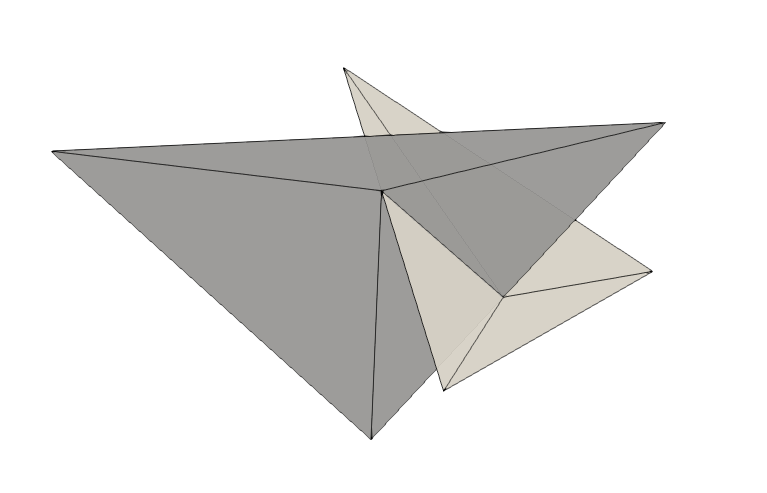
\includegraphics[width=\textwidth]{pics/pic_after_cut.png}
    \caption{Faces after splitting by intersection points.}\label{fig:pic_after_cut}
  \end{minipage}
\end{figure}

After splitting the faces by intersection points, only the following types of relations can remain between the faces of the mesh: two faces do not have common points, two faces have one common vertex, two faces have one common edge.
In this case, new edges that have more than two incident faces appear in our mesh.
If we impose two additional conditions on the original mesh, which can be achieved using local mesh transformations, then we can achieve a fairly simple mesh structure (we will call such meshes simple).
The first condition is the absence of matching vertices in the mesh.
The second condition is that no mesh node is located in any other face.
If these two additional conditions are satisfied, we can state that if an edge has more than two incident faces, then this number is exactly 4, and these 4 incident faces are pairwise in the same plane.

\begin{figure}[h]
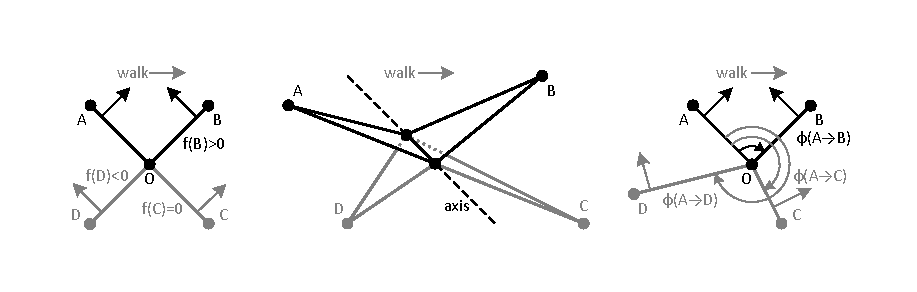
\includegraphics[width=0.85\textwidth]{pics/pic_walk_1_size.pdf}
\captionstyle{center}\caption{Scheme for bypassing the resulting surface.}\label{fig:pic_walk}
\end{figure}

To obtain the resulting surface, it is necessary to get rid of extra faces so that each edge again has exactly 2 incident faces.
To do this, it is necessary to traverse the mesh, starting from any static face, considering two faces adjacent that have a common incident edge (the faces marked during the traversal will be included into the resulting mesh).
When moving from a certain face through an edge that has more than two incident faces, the question arises of choosing a face that should enter the resulting mesh (while all other faces should be deleted).

Consider the procedure for selecting the next mesh walk face for edges with more than two incident faces (Fig.~\ref{fig:pic_walk}, center).
In this figure, the direction of traversal is indicated from left to right, after the face incident with the vertex $A$, the face incident with the vertex $B$ should enter the resulting mesh.
Consider this procedure for simple meshes, as well as for meshes in general.
For simplicity, we will consider the problem in projection onto a plane orthogonal to the edge.

\begin{figure}[h]
  \centering
  \begin{minipage}[h]{0.4\textwidth}
    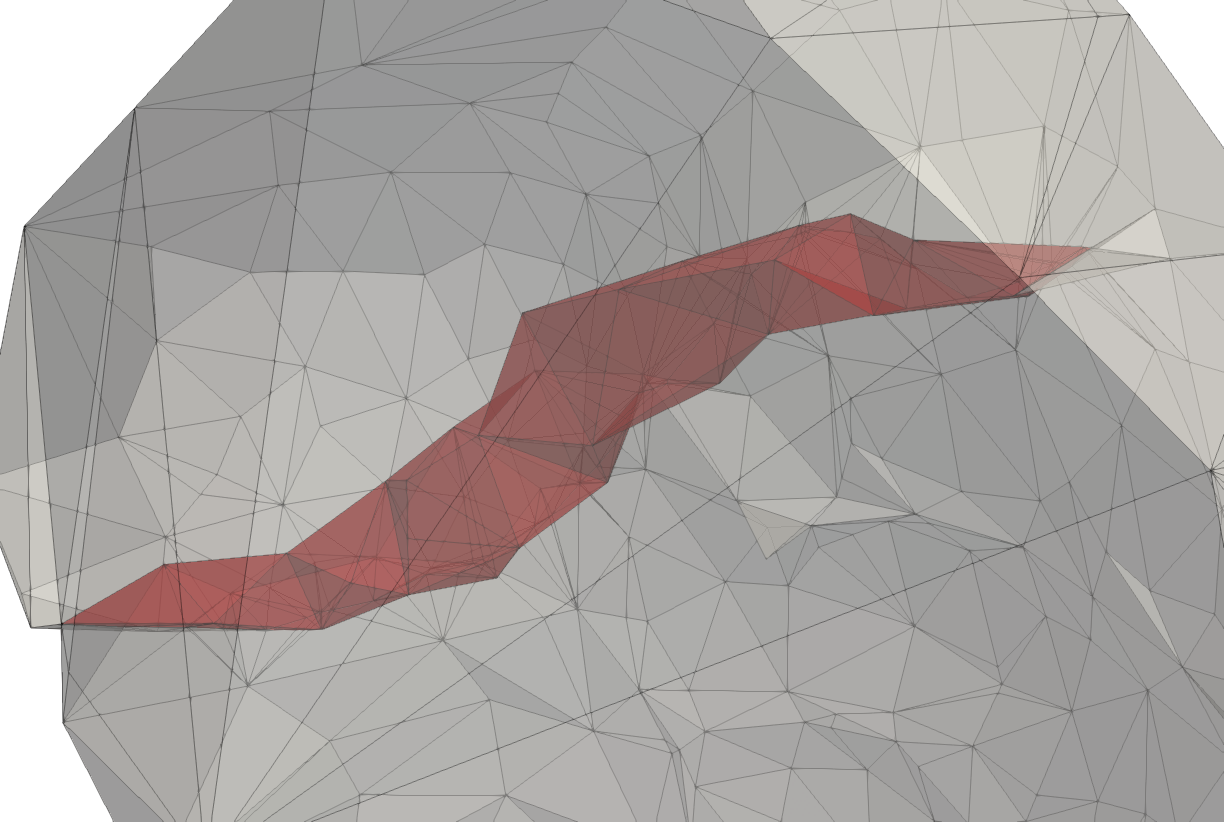
\includegraphics[width=\textwidth]{pics/pic_self_intersection_on.png}
    \caption{The surface before removing the self-intersection.}\label{fig:pic_self_intersection_on}
  \end{minipage}
  \begin{minipage}[h]{0.4\textwidth}
    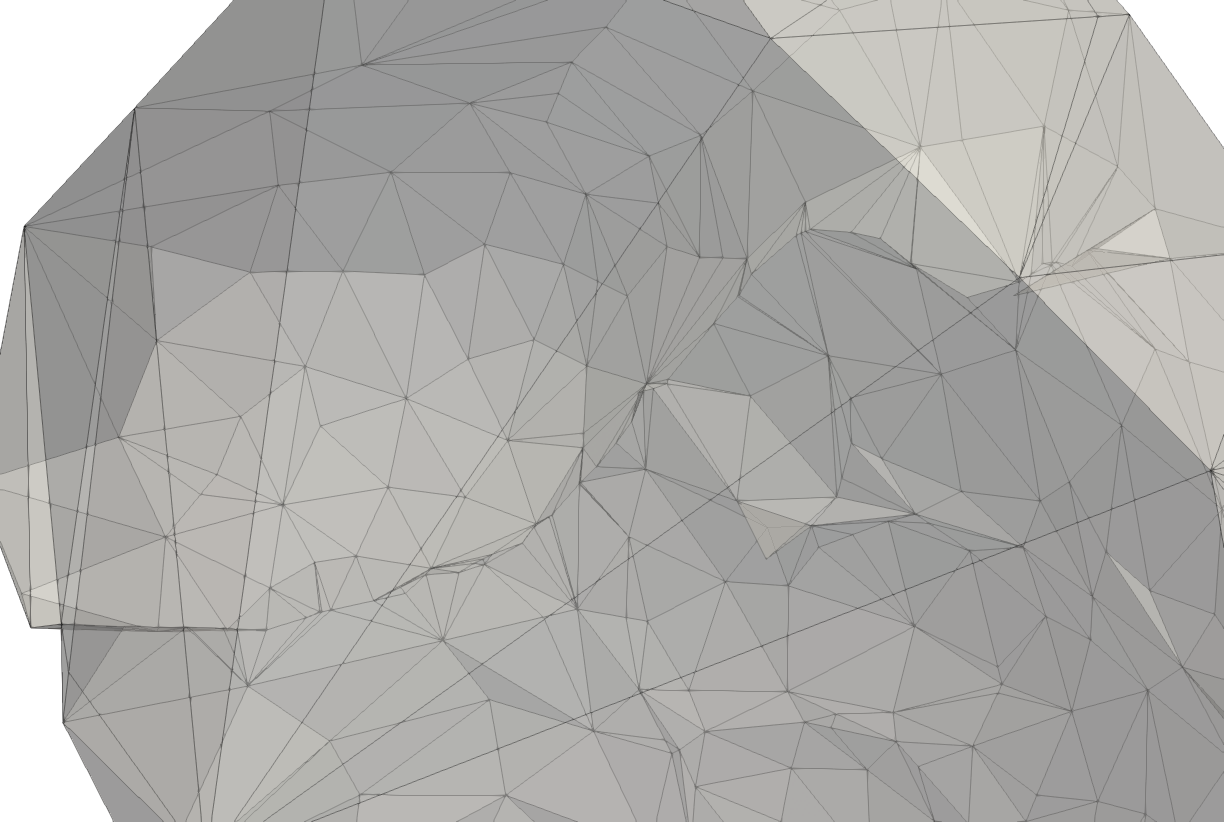
\includegraphics[width=\textwidth]{pics/pic_self_intersection_off.png}
    \caption{The surface after removing the self-intersection.}\label{fig:pic_self_intersection_off}
  \end{minipage}
\end{figure}

\begin{figure}[h]
  \centering
  \begin{minipage}[h]{0.4\textwidth}
    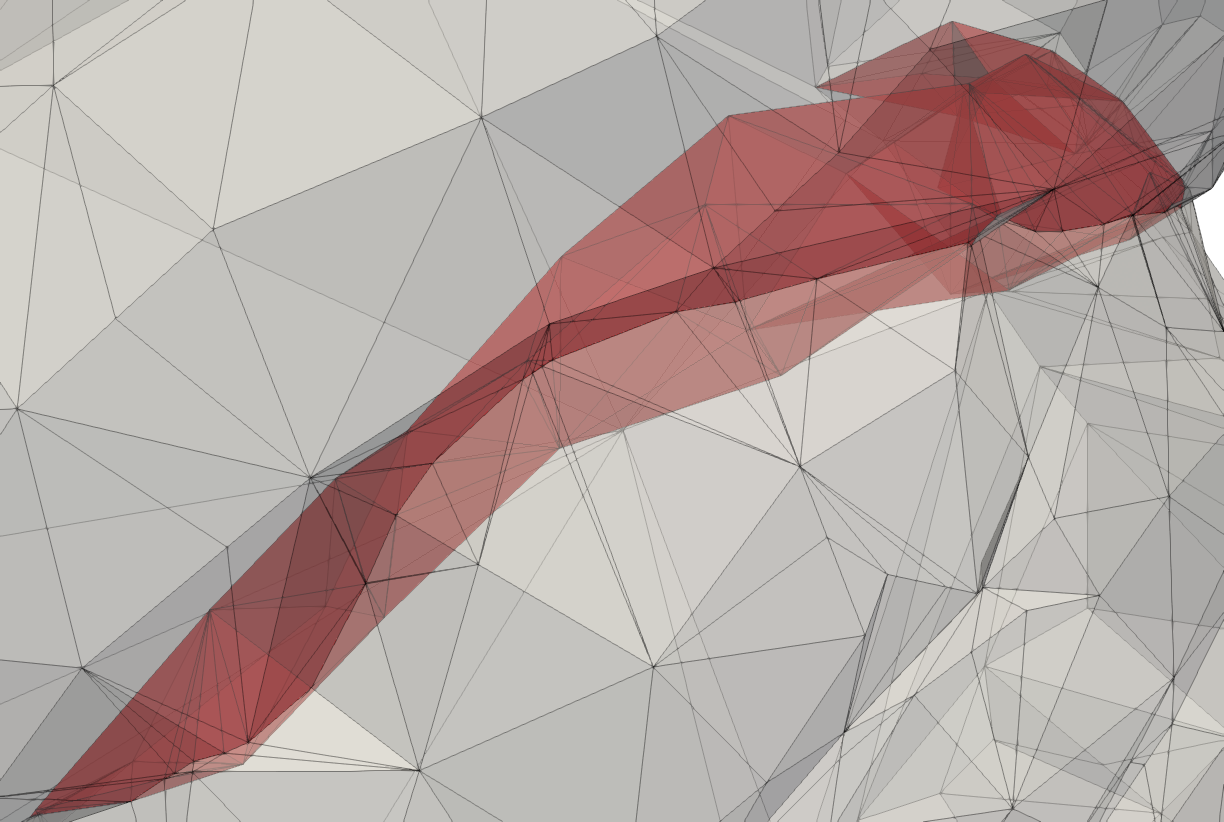
\includegraphics[width=\textwidth]{pics/pic_self_intersection_on_2.png}
    \caption{The surface before removing the self-intersection.}\label{fig:pic_self_intersection_on_2}
  \end{minipage}
  \begin{minipage}[h]{0.4\textwidth}
    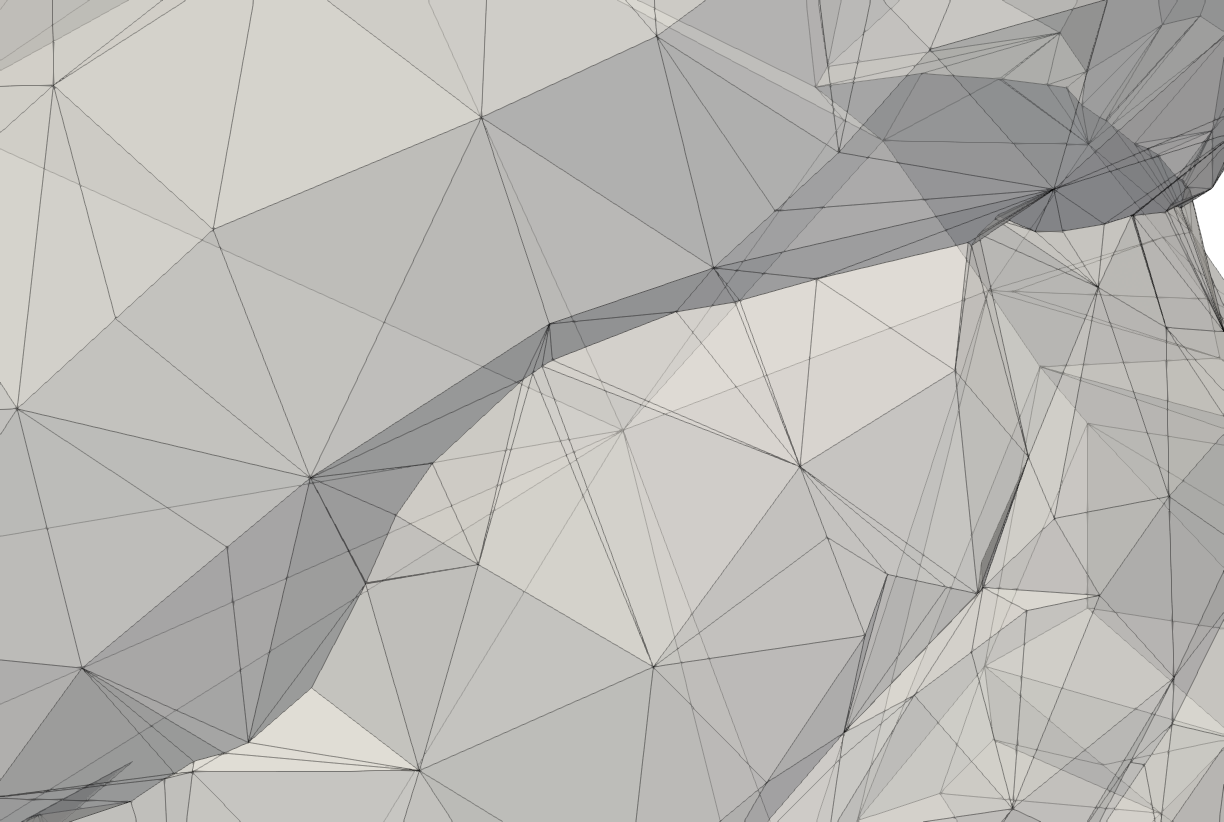
\includegraphics[width=\textwidth]{pics/pic_self_intersection_off_2.png}
    \caption{The surface after removing the self-intersection.}\label{fig:pic_self_intersection_off_2}
  \end{minipage}
\end{figure}

To begin with, we will assume that the case of a simple mesh takes place (Fig.~\ref{fig:pic_walk}, left).
Let it be already known that the face incident to the vertex $A$ is labeled and its outward normal denoted by $\vec{n}_A$.
Of the remaining three faces (incidental to the vertices $B$, $C$, $D$, respectively), it is necessary to choose only one to continue traversing the mesh, and delete the rest.
Since we have a simple mesh, then $\angle AOC = \angle BOD = 2 \pi$, which means $(\vec{n}_A, \vec{OB}) > 0$, $(\vec{n} _A, \vec{OC}) = 0$, $(\vec{n}_A, \vec{OD}) < 0$.
Thus, from all faces, it is necessary to choose the one for which the value of $(\vec{n}_A, \vec{OP})$ is maximum.

Now consider the computational mesh in general case.
In this case, the number of faces incident to the considered edge can be arbitrary, more than two, and nothing can be said about the value of the function $(\vec{n}_A, \vec{OP})$.
To select the next face to bypass the mesh, we will rotate the current face around the considered edge in the direction of $\vec{n}_A$ until it coincides with the first face (Fig.~\ref{fig:pic_walk}, on the right).
The first face must be selected as the next one to continue the mesh traverse.
If we denote by $\phi(A \rightarrow P)$ the angle of rotation of the original face in the direction $\vec{n}_A$ to the face incident with the vertex $P$, then the face for which $\phi(A \rightarrow B)$ will be minimal should be selected as the next one for traverse.

Combining both considered cases together, we obtain  a criterion for
choosing the next face to bypass: a face must be chosen for which
the value of the function $f(P)$ is maximum, where
\begin{equation}
f(P) =
\begin{cases}
(\vec{n}_A, \vec{OP}), \text{for simple meshes}, \\
-\phi(A \rightarrow P), \text{for general case meshes}
\end{cases}
\end{equation}
After completion of the computational mesh bypass, all marked faces are considered to be faces of the target surface, and all other faces must be deleted.
Figures
\ref{fig:pic_self_intersection_on}--\ref{fig:pic_self_intersection_off_2}
illustrate examples of eliminating mesh self-intersections in the
form of hidden loops.
After removing the hidden faces, the target computational mesh again becomes correct, satisfies the relations (\ref{eq_arch}) and can be used for further ice formation modeling.

%---------------------------------------------------------------------------------------------------

\section{Conclusions}

The article considers the geometric aspect of the problem of modeling the ice formation process, namely the problem of the unstructured surface computational mesh evolution.
In the process of evolution, the change in the position of the mesh nodes must correspond to the volume of accumulated ice in the mesh faces, and the mesh itself must remain correct, complete, and not contain self-intersections.
Otherwise, it may not be possible to continue modeling the ice formation process.

The evolution of the computational mesh consists of two main stages.
At the first stage, new positions of mesh nodes are calculated in accordance with the volume of accumulated ice.
A number of the most common algorithms for calculating new node positions were considered, and a new algorithm was proposed.
Among the considered algorithms for calculating new positions of nodes, there were classical algorithms for explicitly calculating the coordinates of nodes, based on the approximation of the ice volume in the form of simple geometric figures (the prisms method and the pyramids method).
A multilayer approach was considered, which simulates iterative ice growth by separate layers, which makes it possible to significantly improve the accuracy of classical methods.
An algorithm for surface rebuilding was considered that uses displacement of vertices while maintaining volume, the main features of which are step-by-step rebuilding, calculation of the maximum proportion of growing ice to prevent local self-intersection, and the use of smoothing of various types to effectively process depressions on the body surface.
A new surface rebuilding algorithm was proposed, based on the formation of a new surface in the form of a common envelope for family of spheres with centers are located on the original surface, and the radii correspond to the intensity of ice growth.
The proposed algorithm is linear in the number of mesh faces, stable, and also tends to close small cracks and depressions on the surface and smooth out sharp peaks and breaks.

Since, regardless of the algorithm used for rebuilding the surface, it is impossible to guarantee the absence of self-intersections of the resulting mesh, the removal of these self-intersections was considered as the second stage of mesh evolution.
Two approaches to eliminating self-intersections were considered.
Both approaches are based on the search for intersections of mesh faces with other faces other than adjacent ones (crossing faces).
The first approach to eliminate self-intersections is to remove the intersection faces and then restore.
As the second approach, we considered a method based on splitting all mesh faces at points of intersection with other faces, bypassing the computational mesh starting from the static area, and removing all unlabeled faces after this bypass.

All considered methods of rebuilding surfaces and eliminating self-intersections were implemented and tested for applicability in ice formation modeling problems.
Based on the results of the testing, a surface rebuilding mechanism based on the common envelope for family of spheres was chosen as a practical use (since this algorithm is fast, reliable, and helps to reduce mesh defects).
As an algorithm for eliminating mesh self-intersections, preference was given to an algorithm based on splitting faces at intersection points.
This algorithm, although rather slow (due to the need to analyze for the intersection of all potentially conflicting pairs of faces), is applicable to computational meshes of arbitrary geometry and complexity.

{\bf Funding.} The work was carried out at the JSCC RAS as part of
the government assignment (topic FNEF-2022-0016). Supercomputer
MVS-10P was used in research.

%---------------------------------------------------------------------------------------------------

\begin{thebibliography}{99}

\bibitem{Raj}
\refitem{article} L.~Prince Raj, K.~Yee, and R.~S.~Myong,
\textquotedblleft Sensivity of  ice and aerodynamic performance
degradation to critical physical and modeling parameters affecting
airfoil icing\textquotedblright, \ Aerospace Science and Technology
{\bf 98}, 105659, 1--46 (2020). DOI: 10.1016/j.ast.2019.105659

\bibitem{Martini}
\refitem{article} F.~Martini, H.~Ibrahim, L.~T.~C.~Montoya, P.~Rizk,
and A.~Ilinca, \textquotedblleft Turbulence  modeling of iced wind
turbine airfoils\textquotedblright, \ Energies {\bf 15}, 8325, 1--21
(2022). DOI: 10.3390/en15228325

\bibitem{Strijhak}
\refitem{article} K.~B.~Koshelev, V.~G.~Melnikova, and S.~V.~Strijhak,
\textquotedblleft Development of iceFoam  solver for modeling ice
accretion,\textquotedblright \ in \textit{Proceedings of the
Institute for System Programming of RAS {\bf 32(4)}, 217--234, 2020}. DOI: 10.15514/ISPRAS-2020-32(4)-16

\bibitem{Sorokin}
\refitem{article} K.~E.~Sorokin, P.~M.~Byvaltsev, A.~A.~Aksenov,
S.~V.~Zhluktov, D.~V.~Savitskiy, A.~A.~Babulin,  and
V.~I.~Shevyakov, \textquotedblleft Numerical simulation of ice
accretion if FlowVision sotfware,\textquotedblright \ Computer
Research and Modeling {\bf 12} (1), 83--96 (2020). DOI: 10.20537/2076-7633-2020-12-1-83-96

\bibitem{Galanov}
\refitem{article}
N.~G.~Galanov, A.~V.~Sarazov, R.~N.~Zhukov, and A.~S.~Kozelkov, \textquotedblleft Application of various ice accretion simulation approaches in the LOGOS software package,\textquotedblright \ Journal of Physics: Conference Series, {\bf 2099}, 012029, 1--8 (2021). DOI: 10.1088/1742-6596/2099/1/012029

\bibitem{Bartkus}
T.~P.~Bartkus, P.~M.~Struk, and J.-C.~Tsao, \textquotedblleft
Evaluation of  a thermodynamic ice-crystal icing model using
experimental ice accretion data,\textquotedblright \ in
\textit{Proceedings of the Atmospheric and Space Environments
Conference, 1--18, 2018}. DOI: 10.2514/6.2018-4129

\bibitem{Zhang}
X.~Zhang, X.~Wu, and J.~Min, \textquotedblleft Aircraft icing  model
considering both rime ice property variability and runback water
effect,\textquotedblright \ International J. of Heat and Mass
Transfer {\bf 104}, 510--516 (2017). DOI: 10.1016/j.ijheatmasstransfer.2016.08.086

\bibitem{Pena}
D.~Pena, Y.~Hoarau, and E.~Laurendeau, \textquotedblleft A  single
step ice accretion model using level-set method,\textquotedblright \
J. of Fluids and Structures {\bf 65}, 278--294 (2016). DOI: 10.1016/j.jfluidstructs.2016.06.001

\bibitem{Beaugendre}
\refitem{misc} H.~Beaugendre, \textquotedblleft A PDE-based approach
to in-flight ice accretion,\textquotedblright \ PhD Thesis (Dep. of
Mech. Eng., McGill Univ., Montr\'eal, Qu\'ebec, 2003).

\bibitem{Rybakov_2D}
\refitem{article} A.~Rybakov and S.~Shumilin, \textquotedblleft
Approximate  methods of the surface mesh deformation in
two-dimensional case,\textquotedblright \ Lobachevskii J. Math. {\bf
40}, 1848--1852 (2019). DOI: 10.1134/S1995080219110258

\bibitem{BourgaultCote}
\refitem{article} S.~Bourgault-C\^ot\'e, K.~Hasanzadeh, P.~Lavoie,
and E.~Laurendeau, \textquotedblleft Multi-layer  icing
methodologies for conservative ice growth,\textquotedblright \ in
\textit{Proceedings of 7th European Conference for Aeronautics and
Aerospace Sciences EUCASS, 1--17, 2017}. DOI: 10.13009/EUCASS2017-258

\bibitem{Thompson}
\refitem{article} D.~Thompson, X.~Tong, Q.~Arnoldus, E.~Collins,
D.~McLaurin, and E.~Luke, \textquotedblleft Discrete  surface
evolution and mesh deformation for aircraft icing
applications,\textquotedblright \ in \textit{Proceedings of the 5th
AIAA Atmospheric and Space Environments Conference, 1--20, 2013}. DOI: 10.2514/6.2013-2544

\bibitem{Tong}
\refitem{article} X.~Tong, D.~Thompson, Q.~Arnoldus, E.~Collins, and
E.~Luke, \textquotedblleft Three-dimensional  surface evolution and
mesh deformation for aircraft icing applications,\textquotedblright
\ J. of Aircraft {\bf 54}, 1047--1063 (2017). DOI: 10.2514/1.C033949

\bibitem{Jiao}
\refitem{article} X.~Jiao, \textquotedblleft Face offsetting: a
unified approach  for explicit moving interfaces,\textquotedblright
\ J. of Computational Physiscs {\bf 220}, 612--625 (2007). DOI: 10.1016/j.jcp.2006.05.021

\bibitem{Jiao_null_space_smooth}
\refitem{article} X.~Jiao, \textquotedblleft Volume and feature
preservation in  surface mesh optimization,\textquotedblright \ in
\textit{Proceedings of the 15th International Meshing Roundtable, 359--373, 2006}. DOI: 10.1007/978-3-540-34958-7\_21

\bibitem{Rivara}
\refitem{article} M.-C.~Rivara and P.~A.~Rodrigez-Moreno,
\textquotedblleft Tuned terminal  triangles centroid Delaunay
algorithm for quality triangulation,\textquotedblright \ in
\textit{27th International Meshing Roundtable, 211--228, 2019}. DOI: 10.1007/978-3-030-13992-6\_12

\bibitem{Rakotoarivelo}
\refitem{article} H.~Rakotoarivelo and F.~Ledoux, \textquotedblleft
Accurate manycore-accelerated  manifold surface remesh
kernels,\textquotedblright \ in \textit{27th International Meshing
Roundtable, 405--423, 2019}. DOI: 10.1007/978-3-030-13992-6\_22

\bibitem{Borouchaki}
\refitem{article} H.~Borouchaki, P.~Laug, and P.-L.~George,
\textquotedblleft Parametric surface meshing using a combined
advancing-front generalized Delaunay approach,\textquotedblright \
International J. for Numerical Methods in Engineering {\bf 49},
233--259 (2000). DOI: 10.1002/1097-0207(20000910/20)49:1/23.0.CO;2-G

\bibitem{Panchal}
\refitem{article} D.~Panchal and D.~Jayaswal, \textquotedblleft
Feature  sensitive geometrically faithful highly regular direct
triangular isotropic surface remeshing,\textquotedblright \
S$\bar{a}$dhan$\bar{a}$ {\bf 47}, 94, 1--19 (2022). DOI: 10.1007/s12046-022-01866-7

\bibitem{Jung}
\refitem{article} W.~Jung, H.~Shin, and B.~K.~Choi,
\textquotedblleft Self-intersection  removal in triangular mesh
offsettings,\textquotedblright \ CAD J. {\bf 1} (1), 477--484
(2004). DOI: 10.1080/16864360.2004.10738290

\bibitem{Freylekhman}
\refitem{article} S.~A.~Freylekhman and A.~A.~Rybakov,
\textquotedblleft Self-intersection elimination  for unstructured
surface computational meshes,\textquotedblright \ Lobachevskii J.
Math. {\bf 43}, 134--140 (2022). DOI: 10.1134/S1995080222130133

\bibitem{Charton}
\refitem{article} J.~Charton, S.~Baek, and Y.~Kim, \textquotedblleft
Mesh repairing using topology graphs,\textquotedblright \ J. of
Computational Design and Engineering {\bf 8}, 251--267 (2021). DOI: 10.1093/jcde/qwaa076

\bibitem{Skvorkovska}
\refitem{article} V.~Skorkovsk\'a, I.~Kolingerov\'a, and B.~Benes,
\textquotedblleft A Simple  and robust approach to computation of
meshes intersection,\textquotedblright \ in \textit{Proceedings of
the 13th International Joint Conference on Computer Vision, Imaging
and Computer Graphics Theory and Applications {\bf 1}, 175--182
(2018)}. DOI: 10.5220/0006538401750182

\end{thebibliography}

\end{document}
